\documentclass[a4paper]{article}
\usepackage[a4paper, total={6in, 9.5in}]{geometry}
\usepackage[utf8]{inputenc}
\usepackage[T1]{fontenc}
\usepackage[UKenglish]{babel}
\usepackage{amsmath}
\usepackage{amssymb}
\usepackage{amsthm}
\usepackage{bm}
\usepackage{booktabs}
\usepackage{float}
\usepackage{graphicx}
\usepackage{hyperref}
\usepackage{listings}
\usepackage{mathpartir}
\usepackage{mathtools}
\usepackage{stmaryrd}
\usepackage{tabularx}
\usepackage{tikz}
\usepackage[t1]{sourcecodepro}
\usepackage[title]{appendix}
\usetikzlibrary{arrows}
\usepackage{enumitem}

% Set globally for all lists
\setlist{itemsep=2pt, parsep=2pt, topsep=3pt}

\definecolor{codegreen}{rgb}{0,0.6,0}
\definecolor{codegray}{rgb}{0.5,0.5,0.5}
\definecolor{codepurple}{rgb}{0.58,0,0.82}
\definecolor{backcolour}{rgb}{0.95,0.95,0.92}

\lstdefinelanguage{Axi}{
  morekeywords=
  {
    module,export,
    from,import,
    primitive,
    forall,
    trait,concept,extends,law,
    instance,
    let,in,
    if,then,else,
    do,
    record,data,type,where,noncomputational,
    induction,match,with,ind,
    theorem,proof,qed,
    assume,
    chaining
  },
  sensitive=true,
  morecomment=[l]{//},     % line comment
  morecomment=[s]{/*}{*/}, % block comment
  morestring=[b]",         % strings in double quotes
  literate=
    {:}{{{\color{codegray}:}}}{1}
    {=}{{{\color{codegray}=}}}{1}
    {=>}{{{\color{codegray}=>}}}{1}
    {|}{{{\color{codegray}|}}}{1}
    {,}{{{\color{codegray},}}}{1}
    {.}{{{\color{codegray}.}}}{1}
    {&}{{{\color{codegray}\&}}}{1}
    {\{\}}{{{\color{codegray}\{\}}}}{1}
    {()}{{{\color{codegray}()}}}{1}
    {->}{{{\color{teal}->}}}{1}
    {<-->}{{{\color{teal}<-->}}}{1}
    {+}{{{\color{teal}+}}}{1}
    {*}{{{\color{teal}*}}}{1}
    {<=}{{{\color{teal}<=}}}{1}
    {==}{{{\color{teal}==}}}{1}
    {===}{{{\color{teal}===}}}{2}
}

\lstdefinestyle{Axi-style}
{
  backgroundcolor=\color{backcolour},
  commentstyle=\color{codegreen},
  keywordstyle=\color{magenta},
  numberstyle=\tiny\color{codegray},
  stringstyle=\color{codepurple},
  basicstyle=\ttfamily\footnotesize\upshape,
  breakatwhitespace=false,
  breaklines=true,
  captionpos=b,
  keepspaces=true,
  numbers=left,
  numbersep=5pt,
  showspaces=false,
  showstringspaces=false,
  showtabs=false,
  tabsize=2
}

\lstset{language=Axi,style=Axi-style}


\lstdefinelanguage{Rust}{
  morekeywords=
  {
    struct,enum,
    type,fn,pub,trait,self
  },
  sensitive=true,
  morecomment=[l]{//},     % line comment
  morecomment=[s]{/*}{*/}, % block comment
  morestring=[b]",         % strings in double quotes
  literate=
    {:}{{{\color{codegray}:}}}{1}
    {;}{{{\color{codegray};}}}{1}
    {,}{{{\color{codegray},}}}{1}
    {&}{{{\color{codegray}\&}}}{1}
    {<}{{{\color{codegray}<}}}{1}
    {>}{{{\color{codegray}>}}}{1}
    {(}{{{\color{codegray}(}}}{1}
    {)}{{{\color{codegray})}}}{1}
    {\{}{{{\color{codegray}\{}}}{1}
    {\}}{{{\color{codegray}\}}}}{1}
}

\newcommand{\code}[1]{{\small \texttt{#1}}}

\title{Khalani: \\ A Next-Generation Blockchain with On-Chain Proofs}
\author{The Khalani Labs Team}
\date{November 2025}

\newtheorem{example}{Example}

\begin{document}

\maketitle

\begin{abstract}
Khalani is an attempt to design and prototype a next-generation blockchain architecture that has the potential to eventually replace the currently dominant Ethereum-style chains. We postulate a collection of novel features for this new blockchain:

\begin{itemize}
  \item purely functional programming on-chain
  \item semantic transparency (there is only one ``canonical'' programming language on-chain --- Axi --- and every on-chain program is bundled with its source code)
  \item resource-aware type system (also known as linear types)
  \item formal logic on-chain (i.e. the ability to formulate and prove theorems and bind them with on-chain programs)
  \item on-chain pub-sub and timers (i.e. proper event-based programming)
  \item support for intent-based programming
  \item code-as-asset (so that code deployed on-chain generates financial profits and can be traded)
  \item account abstraction (ability to programmatically define the behavior of blockchain accounts)
\end{itemize}

We present the details of how these features fit together and how they provide remedies for known problems of existing blockchains. Although some of them are already present elsewhere, the overall vision is new. We conclude with an overview of Axi, Khalani's on-chain programming language.

Caution: this \textit{litepaper} sketches only the key ideas from ongoing research. It is different from the upcoming Khalani \textit{whitepaper}, which will contain detailed technical specifications.
\end{abstract}

\section{Introduction}

\subsection{Timeline of blockchain technology}

Blockchains have been around since 2009 (when Bitcoin was launched). Key milestones include:

\begin{itemize}
  \item 2013 --- understanding that decentralized money could be generalized to a decentralized computer
  \item 2015 --- launch of Ethereum, the first widely adopted decentralized computer platform
  \item 2020 --- the rise of proof-of-stake consensus protocols, promising lower energy use
  \item 2022-2023 --- wider adoption of zk-rollups (e.g., mainnet launches of zkSync Era, Polygon zkEVM), based on the idea of \textit{zero-knowledge proofs}
\end{itemize}

As of 2025, the EVM camp --- consisting of several blockchains compatible with the Ethereum Virtual Machine --- is still dominant as measured by TVL (Total Value Locked).

\subsection{Major obstacles for blockchain adoption}

Despite the overall hype around blockchain technology and cryptocurrencies, the adoption of blockchains remains limited. There are several obstacles hindering wider use.

\subsubsection{Bugs are deadly yet hard to prevent}

Bugs in on-chain programs are extremely costly --- a single smart-contract bug, once exploited by a hacker, can easily destroy the on-chain business that depends on it. However, current methods for preventing bugs are insufficient --- testing cannot guarantee the absence of bugs, and nor can audit. Moreover, once a bug is found, it cannot be fixed, because on-chain programs are immutable by design. Even if a program is explicitly designed to support an upgrade operation (for example, using proxies), this upgrade usually comes too late to prevent losses caused by hackers.

Some examples:

\begin{itemize}
  \item June 2016 --- The DAO exploit (\$50M lost), resulting in the subsequent Ethereum hard fork
  \item November 2017 --- Parity wallets failure (\$150M lost)
  \item August 2022 --- Nomad bridge failure (\$190M lost)
\end{itemize}

\subsubsection{Scammers everywhere}

Because anyone can deploy a program to a public blockchain, users face a core question: which services are trustworthy, i.e. will they actually do what they claim? How can users be confident a service will not steal their funds?

Some examples:

\begin{itemize}
  \item December 2020 --- Compounder Finance (\$10M lost)
  \item October 2021 --- AnubisDAO (\$60M lost)
  \item November 2021 --- Squid Coin (\$3M lost)
\end{itemize}

\subsubsection{``Lost in the maze'' syndrome}

Blockchain technology evolves rapidly. For a typical user, the blockchain space is a maze of chains, services, tokens, credentials, keys, exchanges and responsibilities which becomes increasingly hard to navigate. Although there are numerous efforts to establish community standards (for example, ERC-20 tokens, wallets, DEXes), they do not offset the quickly growing complexity.

\subsubsection{Cross-chain integration}

According to CoinMarketCap, as of November 2025, there are 70 blockchains with market cap exceeding \$1B. The ecosystem does not seem to converge to a single, universal public blockchain and the users have already got used to this diversity of independent chains. This creates integration problems, the first and foremost of which are cross-chain swaps, i.e. moving assets across blockchains.

\subsubsection{Limiting on-chain programming model}

For software developers, blockchains are not nearly as convenient as more traditional computing platforms. The example limitations/difficulties are:

\begin{itemize}
  \item \textbf{The paid-call problem.} To use a given blockchain, a user needs to acquire the native cryptocurrency of this blockchain (in order to pay gas fees). This means the gas mechanics constrain the architecture of dapps. This problem could be mitigated by features like sponsored transactions or delegation.
  \item \textbf{Explicit transaction signing.} Every action taken by a user necessarily takes the form of a transaction, which in turn requires cryptographic signing. Although signing could theoretically be done by any software, this creates a security vulnerability around sharing of private keys. Therefore, users tend to use a single ``trusted'' wallet app for all the signing work, which mitigates sharing risk but on the other hand enforces every act of signing to be a tedious manual interactive process, which, as a result, impairs overall user experience. This could be mitigated if the blockchain programming model supported delegation.
  \item \textbf{Lack of a uniform delegation mechanism.} The previous case is just part of a bigger one: delegation is just not there in blockchains. Say we have Alice (user), Bob, Charlie and Dylan (on-chain services). Bob provides some complicated functionality which involves further interaction with Charlie and Dylan. Alice has no rights to interact with Dylan, so she is forced to use Bob as a privileged intermediary. Charlie recognizes Alice as a user with certain access rights. Bob cannot directly call Charlie because Bob has no rights to do so. Hence Bob would like to interact with Charlie on behalf of Alice and this is exactly the essence of delegation. When Alice wants to ask Bob to do something for her, Bob will have troubles providing a satisfactory level of ``automation'' of actions on behalf of Alice. This is not because such a delegation is fundamentally impossible; rather, the blockchain industry has not agreed on a sufficiently safe and universal mechanism of delegation yet. For example, Ethereum proposals ERC-4337 and EIP-7702 suggest such a universal delegation mechanism that could be added to Ethereum.
  \item \textbf{The ``self-driving taxi paradox''.} Given the currently available autonomous driving technology, combined with wireless Internet access, it is possible to run a taxi service without a driver. However, such a taxi business would face a seemingly trivial problem --- how a car without a driver would refuel itself? So here is the paradox --- a self-driving taxi still needs an operator just to accomplish the gas station interaction. In blockchains we have a similar trouble: services cannot pay for their own gas consumption. Normally, it is the transaction sender who pays gas for the whole transaction execution. This immediately becomes a problem when a service has a common part (say ``a backend'') that from time to time needs to perform some maintenance tasks. These tasks are not performed for a specific user of the service, these tasks are for the service as a whole. But because the service has no way to cover the gas cost of these maintenance activities, the developer of the service has only two solutions available: (1) charge random users during their interaction (2) invoke maintenance whenever needed using a dedicated ``housekeeper'' account. Unfortunately (1) is not reliable (this approach can blow a transaction because of exceeding the gas limit) and not fair, while (2) is even more unreliable because it introduces a dependency on a centralized service. The whole issue could be mitigated by supporting the ``gas reserve'' mechanism.
  \item \textbf{No timers and pub-sub}. Smart contracts cannot natively react to time on-chain events (including in particular clock events, also known as ``timers''). While reactive programming patterns (such as the observer pattern) are standard in off-chain programming, they are not possible on-chain. Because of this, developers have to route reactive processing via off-chain observers, which weakens decentralization.
  \item \textbf{Limited privacy}: Everything on the blockchain is anonymous but public, which is not at all the same thing as privacy. This significantly limits the development of services that critically depend on the privacy of customers' actions. Although it must be said there are some blockchains that attempt to address this problem (for example Zcash and Monero).
\end{itemize}

\subsubsection{The open-source paradox}

Software distribution largely falls into two camps:

\begin{itemize}
  \item \textbf{Commercial software} must be purchased, which funds its creation and maintenance.
  \item \textbf{Open-source software} is free. It is created and maintained by enthusiasts in their spare time. Or by companies that run businesses which depend on transparency.
\end{itemize}

The open-source paradox is this: most of the time open source creators, despite providing crucial value, are not paid for their work. An additional layer of the paradox is that a lot of commercial software depends on open-source software.

In the blockchain world, the situation is even more paradoxical, as there are two dimensions of software to consider:

\begin{itemize}
  \item node software that runs the P2P network
  \item smart contracts that run on-chain
\end{itemize}

In theory node software can be closed-source, but in practice this never happens because transparency is valued so much that only open-source really qualifies for the purpose.

As for on-chain programs, in theory they are not open-source, although they can be easily decompiled and copied because they are visible in the blockchain state. In practice, trust concerns and implied transparency requirements push user preferences towards smart contracts with published source code. Put simply: users won't trust a dapp that does not publish its smart contract source code.

In summary, blockchains lean very strongly towards open-source; monetization is not based on selling or hiding code. Founders most often try to monetize their blockchain via native-asset economics, for example through an Initial Coin Offering. But with more adoption, the blockchain starts running on its own, which means that core on-chain components are developed and maintained by a broader open-source community.

Hence the paradox: the builders who add the most value are not the ones rewarded. On-chain code amplifies this, as it is effectively public by default.

\subsubsection{Integration paths are not well-established (yet)}

Public blockchains are available to anyone, but integrating a blockchain into a business is difficult in practice (except for simple payments), as it is often necessary to hire developers who will design, implement, and deploy a custom dapp. This is an expensive and time-consuming undertaking, bringing its own risks (because of the amount of trust one can put into developers' hands).

Theoretically, the situation could be way better --- we mean just easier integration, without having to build a full dapp. However, this requires the blockchain community to converge on convenient and widely adopted abstractions/standards/APIs. An example of such an abstraction is intent-based processing (which we discuss later). The current state of the convergence is largely insufficient.

\subsubsection{Performance}

Blockchain performance is low. Throughput (measured in transactions-per-second) is constrained by networking and execution. Latency (the delay between transaction sending and its confirmation/finalization) is driven by consensus design and network limits.

This could be improved, for example, if the consensus protocol has some more hints that would decrease the number of state update conflicts.

\subsection{Our mission}

We aim to prototype a next-generation blockchain. Our main focus is on the on-chain programming model, i.e. the Virtual Machine (VM). We pair a novel and innovative VM design with some existing performant proof-of-stake consensus protocol.

We hope that the adoption of Khalani will challenge EVM dominance by offering significant usability gains and that, as a consequence, its ideas will spread to other chains, inspiring innovation and moving the industry forward.

The key distinguishing features of the Khalani blockchain are:

\begin{itemize}
  \item Axi, a \textbf{purely functional} programming language for smart contracts
  \begin{itemize}
    \item type system based on linear logic/quantitative type theory (also known as ``programmable assets'')
    \item on-chain formal logic for proving theorems about smart contracts
    \item concepts (infrastructure that combines interfaces with formal specifications; in other words, combines programming and logic into a convenient flow of ``semantic interfaces'')
  \end{itemize}
  \item native support for \textbf{intents} and \textbf{delegation}
  \item on-chain events system (\textbf{pub-sub} and timers)
  \item \textbf{gas reserve} mechanism
  \item native \textbf{account abstraction}
  \item \textbf{code-as-asset} (code you wrote earns money for you, code is an asset and can be traded)
\end{itemize}

The following table gives a bird's-eye overview of key blockchain adoption obstacles (as listed above) vs features of Khalani blockchain that are supposed to mitigate them.

\bigskip
\begin{tabularx}{\textwidth}{|l|X|}
\hline
\textbf{Problem} & \textbf{Khalani's solution} \\
\hline
Bugs (exploited by hackers) & Khalani smart contracts are written in Axi, a purely functional programming language. Axi supports so-called ``concepts'' (concept is a language feature in Axi) which are semantically-enriched interfaces. In Axi one can use formal logic to prove that a software component is compliant with a given concept.

The economic incentives are arranged in a way that both the concept developers are rewarded for creation of popular concepts and dapp developers are rewarded for proving compliance with concepts.

We believe the existence of concepts will generate social pressure on developers, as the reputation of their dapps will depend on the compliance with well-established concepts. The source of the pressure will come from users --- because the concepts infrastructure will surface at end-user level (for example in the form of easy-to-see badges, similar to how easily people use SSL in a web browser by having the lock icon there). \\
\hline
Scams and frauds & Code in a purely functional programming language is very transparent, making it harder to obfuscate what a smart contract actually does. Formal logic provides an effective way to express formal guarantees. Checked proofs are part of the blockchain state agreed upon by consensus. \\
\hline
Lost in the maze syndrome & Intent-based processing \\
\hline
Cross-chain integration & Intent-based processing \\
\hline
Delegation mechanism is missing & Delegation mechanism. \\
\hline
Self-driving taxi paradox & Gas reserve. \\
\hline
No on-chain timers & In-protocol support for timers. \\
\hline
No on-chain pub-sub & In-protocol support for pub-sub. \\
\hline
Open-source paradox & Code-as-asset \\
\hline
Integration paths not well-established & Economic incentives to build and converge around common abstractions (concepts), implemented in Axi as concepts. \\
\hline
Performance & UTXO consensus, which is based on a partial order (as opposed to a sequence), with declared inputs of every transaction. Also, the object ownership model reduces collisions between transactions. \\
\hline
Limited privacy & For now the relevant features of Khalani are not decided yet. We are looking into existing solutions (such as Monero and Zcash) to estimate feasibility. \\
\hline
\end{tabularx}
\bigskip

\subsection{Sources of inspiration}

The \href{https://sui.io/}{Sui} blockchain was the main inspiration behind our ledger structure and the use of linear types. We also extensively studied UTXO-based blockchains (\href{https://www.nervos.org/}{Nervos} and \href{https://cardano.org/}{Cardano}) to understand their advantages and limitations.

When designing Axi, our guiding principle was \href{https://en.wikipedia.org/wiki/Intuitionistic_type_theory}{Intuitionistic Type Theory}. The logical features were inspired by proof assistants such as \href{https://rocq-prover.org/}{Coq} and \href{https://lean-lang.org/}{Lean}, whereas the programming side drew inspiration from languages like \href{https://www.haskell.org/}{Haskell} (the general spirit) and \href{https://www.unison-lang.org/}{Unison} (regarding optimal blockchain-aware source code representation). Earlier we rejected an approach based on \href{https://people.csail.mit.edu/kostas/dpls/dpl-dissertation.pdf}{Denotational Proof Languages} and the \href{https://athena-lang.org/learn}{Athena proof system}.

We also spent time reviewing the current state of intent-based processing ideas:

\begin{itemize}
  \item \href{https://eips.ethereum.org/EIPS/eip-7521}{https://eips.ethereum.org/EIPS/eip-7521}
  \item \href{https://anoma.net/}{https://anoma.net/}
  \item \href{https://docs.essential.builders/welcome/}{https://docs.essential.builders/welcome/}
\end{itemize}

The ideas behind delegation, mandarins, on-chain timers and pub-sub, gas reserve and code-as-asset are our own inventions.

\section{Ingredients of the architecture}

\subsection{Axi}

\subsubsection{Functional programming with formal logic built-in}

In \textbf{imperative programming}, the most widespread programming paradigm, the role of the program is to modify the computer's memory. The program is composed of a bunch of statements. The most basic statement is variable assignment. Assignments are then combined into more complex programs using loops, conditionals and procedure definitions. Execution of the program proceeds statement by statement, at every step modifying chunks of memory. When the execution is complete, the transformation of the computer's memory described by the program has been carried out.

\textbf{Functional programming} is a programming paradigm in which a program is constructed as a composite expression that defines a single function. The primordial building blocks of functional programming are:

\begin{itemize}
  \item defining functions
  \item application (invoking a function on given arguments)
  \item pairing (constructing tuples)
  \item pattern matching
\end{itemize}

An important part of the functional paradigm is a rich type system, which allows for algebraic data types and functional types. The assignment statement is not supported (not needed); it is only possible to define constants.

Functional programming has one advantage over imperative: it is easier to reason about functional programs, in particular when doing reasoning with formal logic. This was the key reason why we decided to adopt the functional approach to on-chain programming in Khalani.

\textbf{Axi} is a purely functional programming language we designed from scratch. Axi borrows key ideas from type-theoretical proof assistants like Coq, Lean and Agda. These languages are purely functional (like Haskell) but with an added superpower --- they include formal logic. Hence, in Axi one can implement programs and also prove theorems about these programs.

\subsubsection{Concepts}

Axi merges programming and logic via \textbf{concepts}. A concept bundles together declarations of constants, functions, abstract types, and logical statements about them. It can be understood as a ``semantically enriched'' interface. Concepts serve as the mechanism for transporting logic to the programming layer.

Concepts can capture high-level on-chain concepts such as DEX, bridge, swap, and escrow. We expect a growing library of such concepts to develop organically over time, thus encouraging convergence on common abstractions needed for integration.

\subsubsection{Linear types}

Linear types enforce that a value is used exactly once, thus allowing the type system to establish the idea of ``resources'' at the programming level. This lets developers:

\begin{itemize}
  \item safely deallocate an object after its use
  \item design software interfaces that guarantee a resource cannot be used after it has been closed or transitioned to a different state
\end{itemize}

While brewing since the '80s, linear types have been popularized around 2012 when they appeared as the core concept in the \href{https://en.wikipedia.org/wiki/Rust_(programming_language)}{Rust} programming language. In 2018, this idea was adopted by the \href{https://move-book.com/}{Move} programming language, where linear types are the way to keep track of \textbf{resources} during program execution. This neatly fits into the on-chain money abstraction.

Move underpins Sui and Aptos, demonstrating the power of linear typing for building blockchain abstractions. This is why we decided to adopt linear typing in Axi.

\subsubsection{Semantic transparency}

In traditional blockchains (such as Ethereum), code of on-chain programs is stored in its compiled form, in the bytecode format (low-level representation using the internal language of the VM). This approach resembles traditional computers, where the CPU executes machine code, while developers use various programming languages which are compiled to machine code. The biggest advantage of this approach is the freedom of choice of the smart-contract programming language. The biggest disadvantage is that smart-contracts are hard to understand and analyze.

In Khalani, we adopt the opposite extreme: we enforce that all the on-chain code must be written in Axi. Moreover, we actually store on-chain the source code of Axi programs. Precisely speaking, code is stored as content-addressed elaborated AST:

\begin{itemize}
  \item \textbf{AST} stands for ``abstract syntax tree''; it is just the result of parsing the textual sources
  \item \textbf{content-addressed}: this means that code is stored as a large key-value structure, where the key is the cryptographic-digest (i.e. hash) of the value, and the value is a corresponding chunk of code (an expression or a declaration)
  \item \textbf{elaborated}: this is a form where the AST is enriched with the results of the type-checking; in this form, the types of all expressions are inferred and explicitly included as type annotations
\end{itemize}

The advantage of the elaborated form of the source code is that it can be formally verified in linear time (while the type-checking of the original source code could be exponential-time). This way we shield ourselves from certain kinds of DoS attacks.

Using source code as the ``master copy'' stored on-chain (instead of the bytecode) means that we deliberately sacrifice freedom of programming language choice in favor of \textbf{semantic transparency}: all the on-chain code is apparent, high-level, type-safe, easy to understand and homogeneous in its form. All the typing information is preserved, all the names and comments are there. There is no obfuscation caused (naturally) by the compilation process. Keep in mind that Axi code also includes theorems and proofs --- they are also preserved and fully available on-chain.

Of course, the compilation of Axi code is eventually needed for its execution. Code will get compiled at the node level, so that a node can execute transactions. However, we consider this to be the node's implementation detail. Nodes will have freedom to use different Axi compilers, or even stick to an interpreter --- as long as they respect the execution semantics of Axi (which is formally specified). Nodes can also cache the compiled versions of Axi packages to speed up execution.

\subsection{Ledger model}

\subsubsection{UTXO and state evolution}

Global state (``current state of the world'') in Khalani blockchain is composed of two parts:

\begin{itemize}
  \item \textbf{data zone}: this part follows the UTXO structure (cells)
  \item \textbf{code zone:} this part contains executable programs arranged into packages/modules
\end{itemize}

The global state evolves by executing transactions. A transaction can consume some cells, read some cells, create some cells and deploy some packages. The following pseudocode specifies the structure of the ledger model in a more detailed way:

\begin{lstlisting}[language=Rust]
struct Cell<T> {
  address: Address,
  payload_type: (package: &Package, module: String, struct: String),
  version: Long,
  payload: T,
  kind: CellKind,
  status: CellStatus
}

struct Package {
  address: Address,
  modules: Vec<Module>
}

enum CellStatus {
  Alive,
  Dead
}

enum CellKind {
  Shared,
  Private,
  Immutable,
  Account
}

struct ExecutedTransaction {
  protocol_version: Long,
  nonce: Nonce,
  transactor: Address,
  epoch: Long,
  consumed_gas: Gas,
  gas_price: GasPrice,
  inputs: Vec<(Address, InputMode)>,
  outputs: Vec<Address>,
  deploys: Vec<Package>,
  txid: Hash
}

enum InputMode {
  ReadOnly,
  Update,
  Delete
}
\end{lstlisting}

Cell identity is represented by its address. Each address has a linear version history. \code{ReadOnly} is a special read-only input mode in which the cell is not consumed (we also call such read-only input cells `dependencies'; this is the traditional term used in Nervos). Cells read with input mode \code{Delete} switch status to \code{Dead}. Cells read with input mode \code{Update} also switch status to \code{Dead}, and a modified copy (same address and type, incremented version) is created among the outputs.

Every cell is typed (with an Axi type) and contains exactly one value (i.e. an object) of that type --- this value is kept in the field \code{payload}. The type is set at the cell's creation and cannot change during its lifetime. In other words, cell updates preserve the cell's payload type. We will simply say ``cell's type'' when we mean cell's payload type.

A cell's kind is another concept (not to be confused with the cell's type) which we discuss later in the sub-chapter \textbf{Cell kinds and ownership}.

To capture the intuition behind the model we show it below with a couple of pictures (for the pictures the model is somewhat simplified). The conventions are:

\begin{itemize}
  \item 3-byte hashes as cell addresses
  \item 4-byte hashes as transaction identifiers
  \item \code{0a3f11/1} denotes version \code{1} of the cell at address \code{0a3f11}
  \item cell types are shown as simple names (for example \code{Coin} is the name of cell's type)
  \item cell kinds are not shown
  \item package deploys are not present in this example
  \item alive cells are green
  \item dead cells are red
  \item solid black lines represent cell consumption/creation
  \item solid blue lines represent cell update
  \item dotted lines represent cell reading (i.e. \code{input-mode=ReadOnly})
\end{itemize}

Suppose we started with four live cells:

\begin{figure}[H]
  \centering
  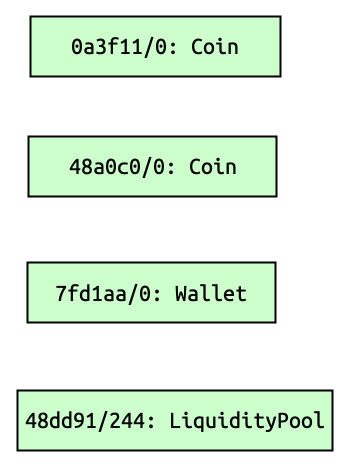
\includegraphics[width=0.2\textwidth]{graphics/ledger-1.png}
\end{figure}

Then the transaction \code{e823fa01} is executed. It has two inputs and one output. Cell \code{0a3f11} gets updated (so a new version of it is created). Cell \code{48a0c0} gets consumed (i.e. destroyed):

\begin{figure}[H]
  \centering
  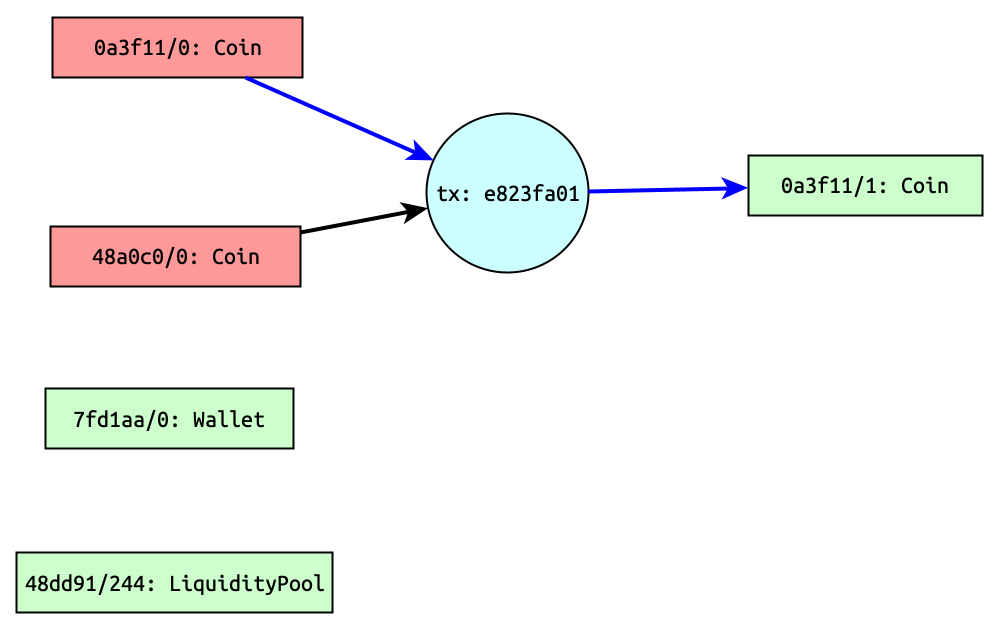
\includegraphics[width=0.8\textwidth]{graphics/ledger-2.png}
\end{figure}

Then the transaction \code{42d1e035} is executed. It has one dependency, one consumption and three outputs:

\begin{figure}[H]
  \centering
  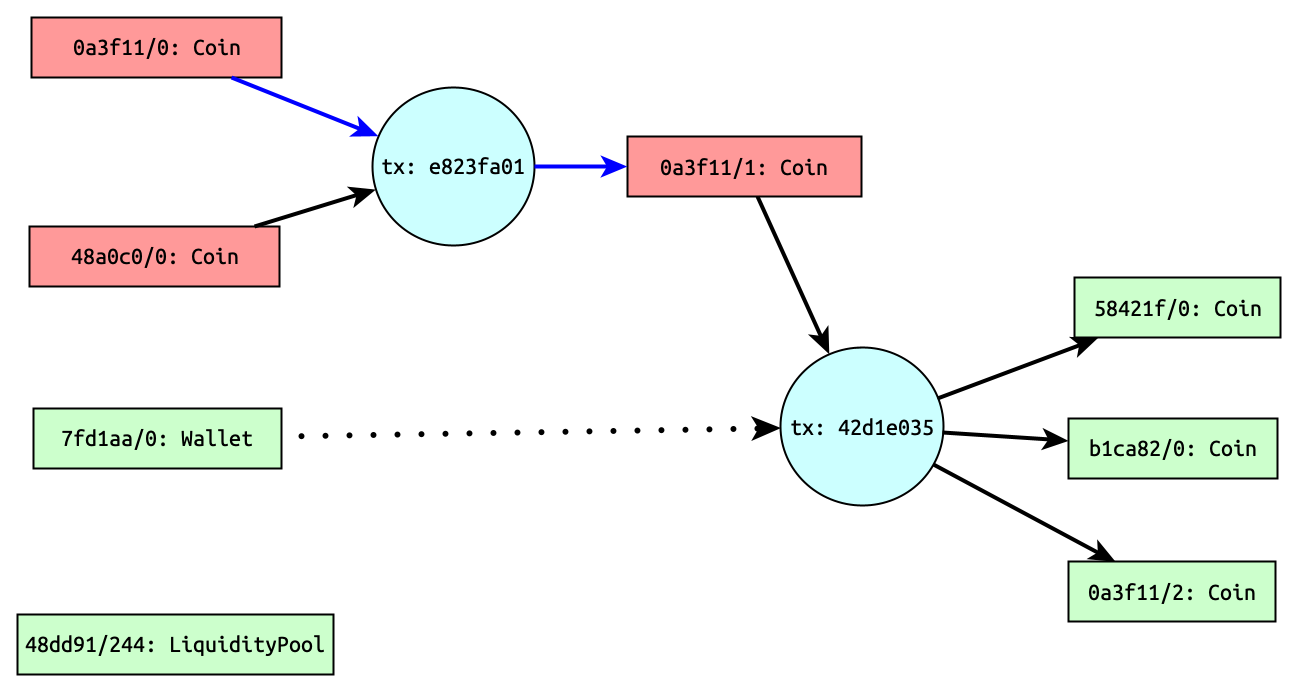
\includegraphics[width=\textwidth]{graphics/ledger-3.png}
\end{figure}

Then the transaction \code{155e0a90} is executed. It has three inputs and one output:

\begin{figure}[H]
  \centering
  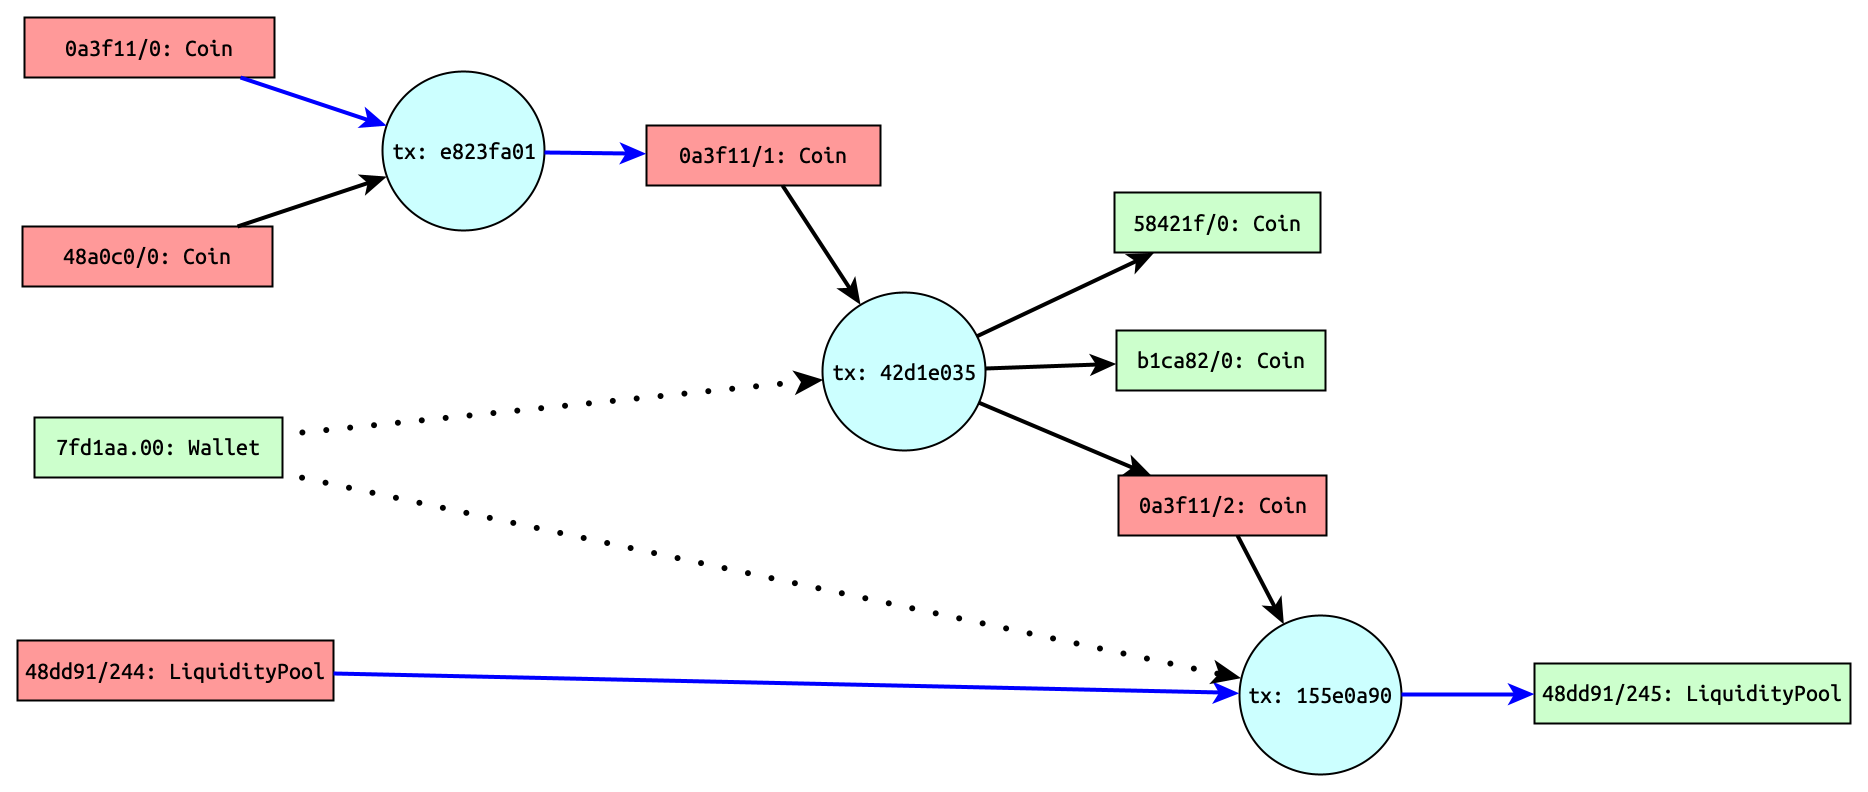
\includegraphics[width=\textwidth]{graphics/ledger-4.png}
\end{figure}

The ledger grows indefinitely, forming a Directed Acyclic Graph (DAG) which might look like this:

\begin{figure}[H]
  \centering
  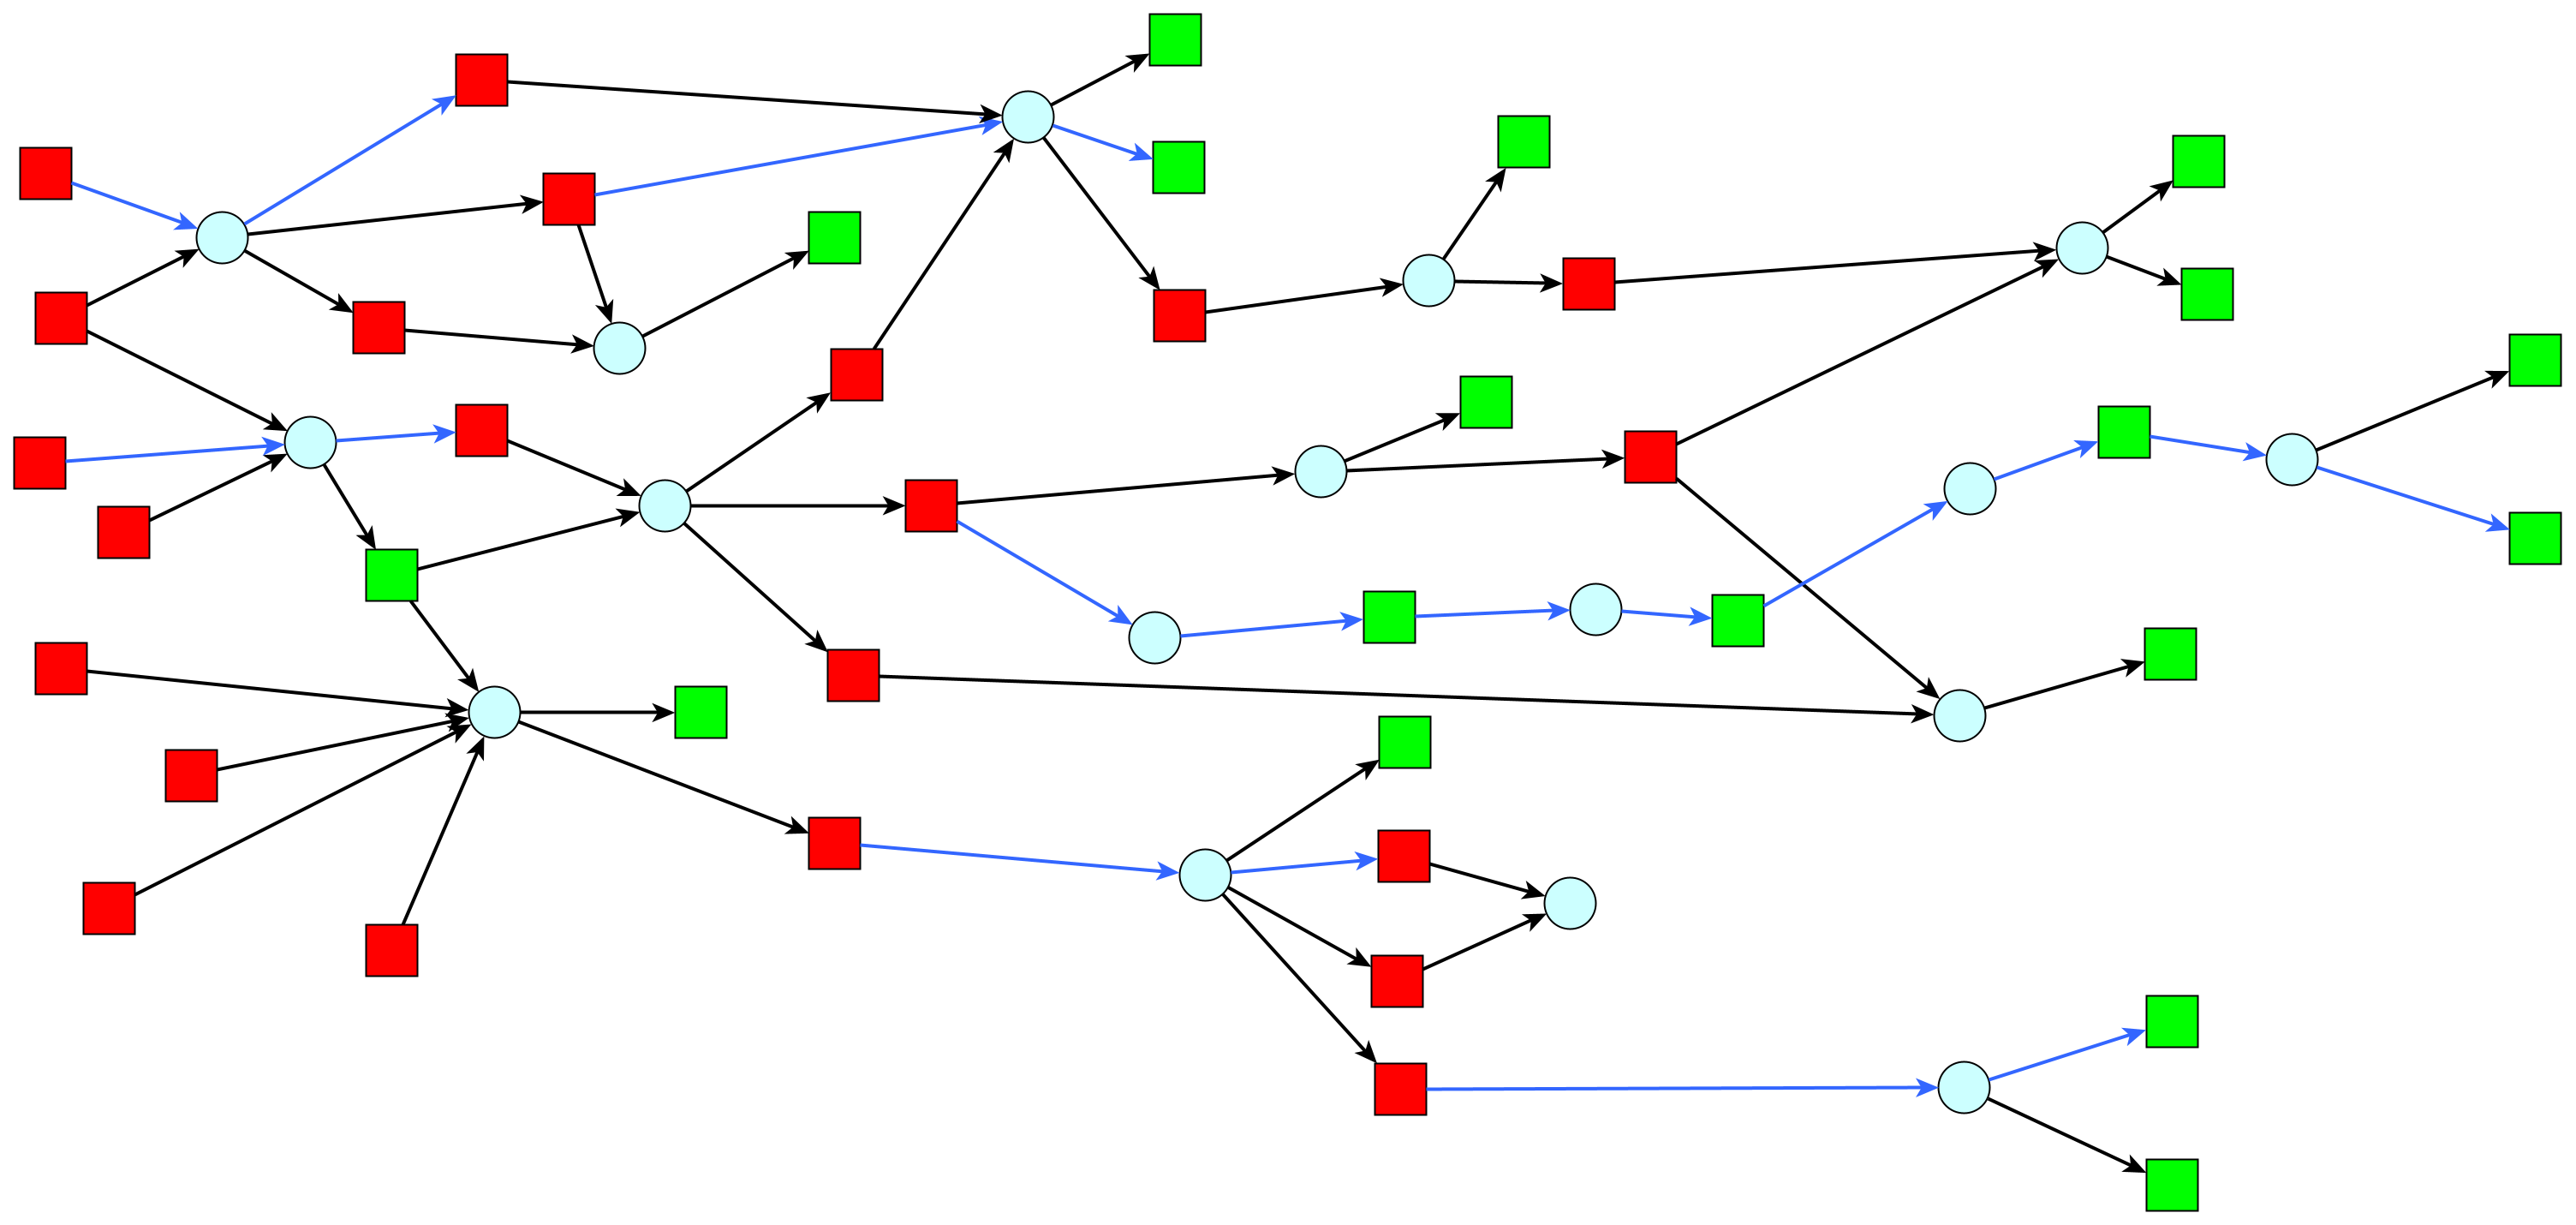
\includegraphics[width=\textwidth]{graphics/long-ledger.png}
\end{figure}

The set of live cells is what we call ``the current global state''. It represents the latest state of the blockchain's memory.

\subsubsection{Packages, modules and imports}

On-chain code is organized into packages and modules. Packages are much like cells --- every transaction can deploy a package (or a collection of packages). Every package is public. Packages are immutable and permanent, i.e. once deployed, they cannot be changed in any way and they stay on-chain forever. There is no package ``upgrade'' mechanism and no package versioning. Deploying a modified version of an existing package yields a new independent package with a new hash. A package is just a public shared library and the blockchain itself can be seen as a decentralized repository of Axi packages.

A package contains a hierarchy of modules (identified by their hierarchical names). Each module serves as a namespace and contains Axi code: types, constants, functions, traits, theorems and proofs. Modules can import selected definitions from public modules of their enclosing package and also from public modules of other (previously deployed) packages.

Axi source code is stored on-chain as an AST (abstract syntax tree). Nodes of the AST are content-addressed by cryptographic hashes, so duplication is impossible. In particular, the package itself is addressed by the hash of its contents.

\subsubsection{Where are the smart contracts?}

The reader may be surprised we have not mentioned smart contracts yet, while they otherwise seem to be a ubiquitous concept in the blockchain industry. Let us explain our reasons.

Historically, the common understanding of what a smart contract is, has been established in the technological context of Ethereum. Ethereum has two types of accounts (we ignore here the latest ERC-4337 addition of so-called ``smart accounts''):

\begin{itemize}
  \item externally owned accounts (EOA)
  \item smart-contract accounts (SCA)
\end{itemize}

The model of Ethereum was heavily inspired by object-oriented programming ideas, so the semantics of account types can be explained in the following way:

\begin{itemize}
  \item the blockchain is a computer
  \item EOAs represent users (and are just cryptographic key-pairs, used for signing transactions)
  \item SCAs represent programs (and operate as if being standalone mutable objects)
\end{itemize}

Inside an SCA, data and code operating on this data are bundled together, i.e. exactly like in a singleton object in any object-oriented programming language. Because public methods of an SCA form an API that other SCAs (and transactions) can call, it can also be seen as a small ``server'' operating on-chain.

However, in most object-oriented programming languages, classes and instances are concepts living on different levels: classes contain code, while objects contain data. This way, a class serves as a template for objects. Several instances of a class can be created, all of these instances --- called objects --- sharing the same behavior. Meanwhile in the Ethereum model the class-objects separation is not properly reflected: there are no classes. An SCA is like a singleton object glued together with its class.

This problem can be easily fixed, though --- it would be sufficient to detach code from objects, i.e. have objects and classes as separate concepts in the VM. But when you follow this idea, the concept of a ``smart contract'' does not fit the situation anymore.

This is exactly what we do in the Khalani blockchain:

\begin{itemize}
  \item code is in modules
  \item data is in cells
  \item every cell contains a single object --- this object is an instance of its ``class''; however, because Khalani on-chain programming is really functional programming in Axi, we rather say that this object is an element of its type (where the definition of the type sits in some module)
\end{itemize}

Smart contracts from Ethereum can be ported to the Khalani blockchain --- every smart contract would then correspond to a shared cell (here ``shared'' is a so-called \textbf{kind} of cell --- we describe kinds later in the next chapter). We just do not use the term ``smart-contract'' for a shared cell because the code defining the structure and behavior of the cell is not part of the cell (instead it is defined by functions in the corresponding module). We also do not want to use the term ``smart-contract'' meaning the module, because this could create even bigger confusion for people used to the Ethereum model (because in Khalani the closest thing to Ethereum smart contracts are really shared cells).

\subsubsection{Cell kinds and ownership}

Every cell has a \textbf{kind}, which is one of:

\begin{itemize}
  \item \textbf{private} --- this means it is owned by an account (has restricted access)
  \item \textbf{shared} --- it means it is mutable and accessible to everyone
  \item \textbf{immutable} --- it means it is immutable and accessible to everyone
  \item \textbf{account} --- it is a special cell that represents blockchain user identity
\end{itemize}

An account is a special kind of a cell --- we need it to implement account abstraction (see the \textbf{Accounts} chapter for more details on this).

Shared cells are the way to implement ``services''.

Immutable cells are for storing public data on-chain. They can be used as stateless services.

Private cells are mostly useful as envelopes for resources (such as cryptocurrencies). They can be owned by accounts --- for convenience. For example, an account can point to the address of a cell containing money to be used for covering gas. Shared cells cannot own private cells, because they can more easily store their resources directly inside the master cell.

\subsubsection{Cell usage patterns}

The blockchain cell-based model is very flexible and it is not desirable (or even possible) to enumerate up-front all the software patterns that developers will come up with over time. But we wanted to mention four such patterns:

\begin{itemize}
  \item service
  \item asset container
  \item account
  \item mandarin
\end{itemize}

A \textbf{service} is a pattern that effectively resembles smart-contract accounts from Ethereum: there is an on-chain object sitting at a fixed well-known address and offering a public interface to be called by other on-chain actors (objects and accounts). An example of such a service could be a DEX, a bridge, a name-registration service, an oracle, or a facade to an on-chain economic game.

An \textbf{asset} pattern is for creating generally ``passive'' resources which can be traded/purchased: cryptocurrencies, NFTs, wrapped coins, soul-bound tokens. A built-in cryptocurrency of Khalani is also materialized using the asset pattern.

A \textbf{mandarin} pattern is the one we promote for intent-based processing. We introduce it later in the document.

An \textbf{account} is a special type of cell to support account abstraction (it is required to implement a dedicated interface that is recognized by the VM).

\subsection{Accounts}

\subsubsection{Motivations}

In a traditional blockchain like Ethereum, an account is established as a public-private pair of cryptographic keys. Then the pair serves two purposes at once:

\begin{itemize}
  \item the hash of the public key becomes the account's address
  \item the key pair is used to form cryptographic signatures of transactions
\end{itemize}

The on-chain representation of an account is then managed by the VM and it holds:

\begin{itemize}
  \item native cryptocurrency balance
  \item latest nonce (in order to control transactions ordering)
\end{itemize}

This approach is simple and efficient but it has limitations. For example one cannot:

\begin{itemize}
  \item implement multi-sig schemes (threshold cryptography)
  \item implement cryptographic key management (so that there are many keys used to sign transactions for a single account, while the list of the active keys can be managed)
  \item implement per-key privileges configuration
  \item customize the transaction binary format (serialization)
  \item customize tx-level API for his account (for example allowing certain fixed set of operations only)
\end{itemize}

These problems are not new and can be summarized in a simple way: every account works in exactly the same way, a way that is sealed into the blockchain protocol.

The opposite approach is to allow programmable accounts. This is otherwise known as \textbf{account abstraction}.

\subsubsection{Our approach to account abstraction}

As we already explained, our cells play the role analogous to smart-contracts. A cell's behavior is determined by the type of the object it contains.

Therefore, not surprisingly, our account abstraction is based on \textbf{account objects}, but we will actually use the term \textbf{account} for talking about account objects. Like any other object, an account is programmable. An account object lives in a dedicated mutable cell, hence it has an address. This address is otherwise known as the \textbf{account address}.

The VM recognizes accounts as ``special'' cells: they play the role of ``gatekeepers'' for the whole blockchain. Specifically --- every incoming transaction gets interpreted by the corresponding account. ``Interpreted'' means that it is the account that decides how this transaction is going to be executed --- if at all.

\begin{figure}[H]
  \centering
  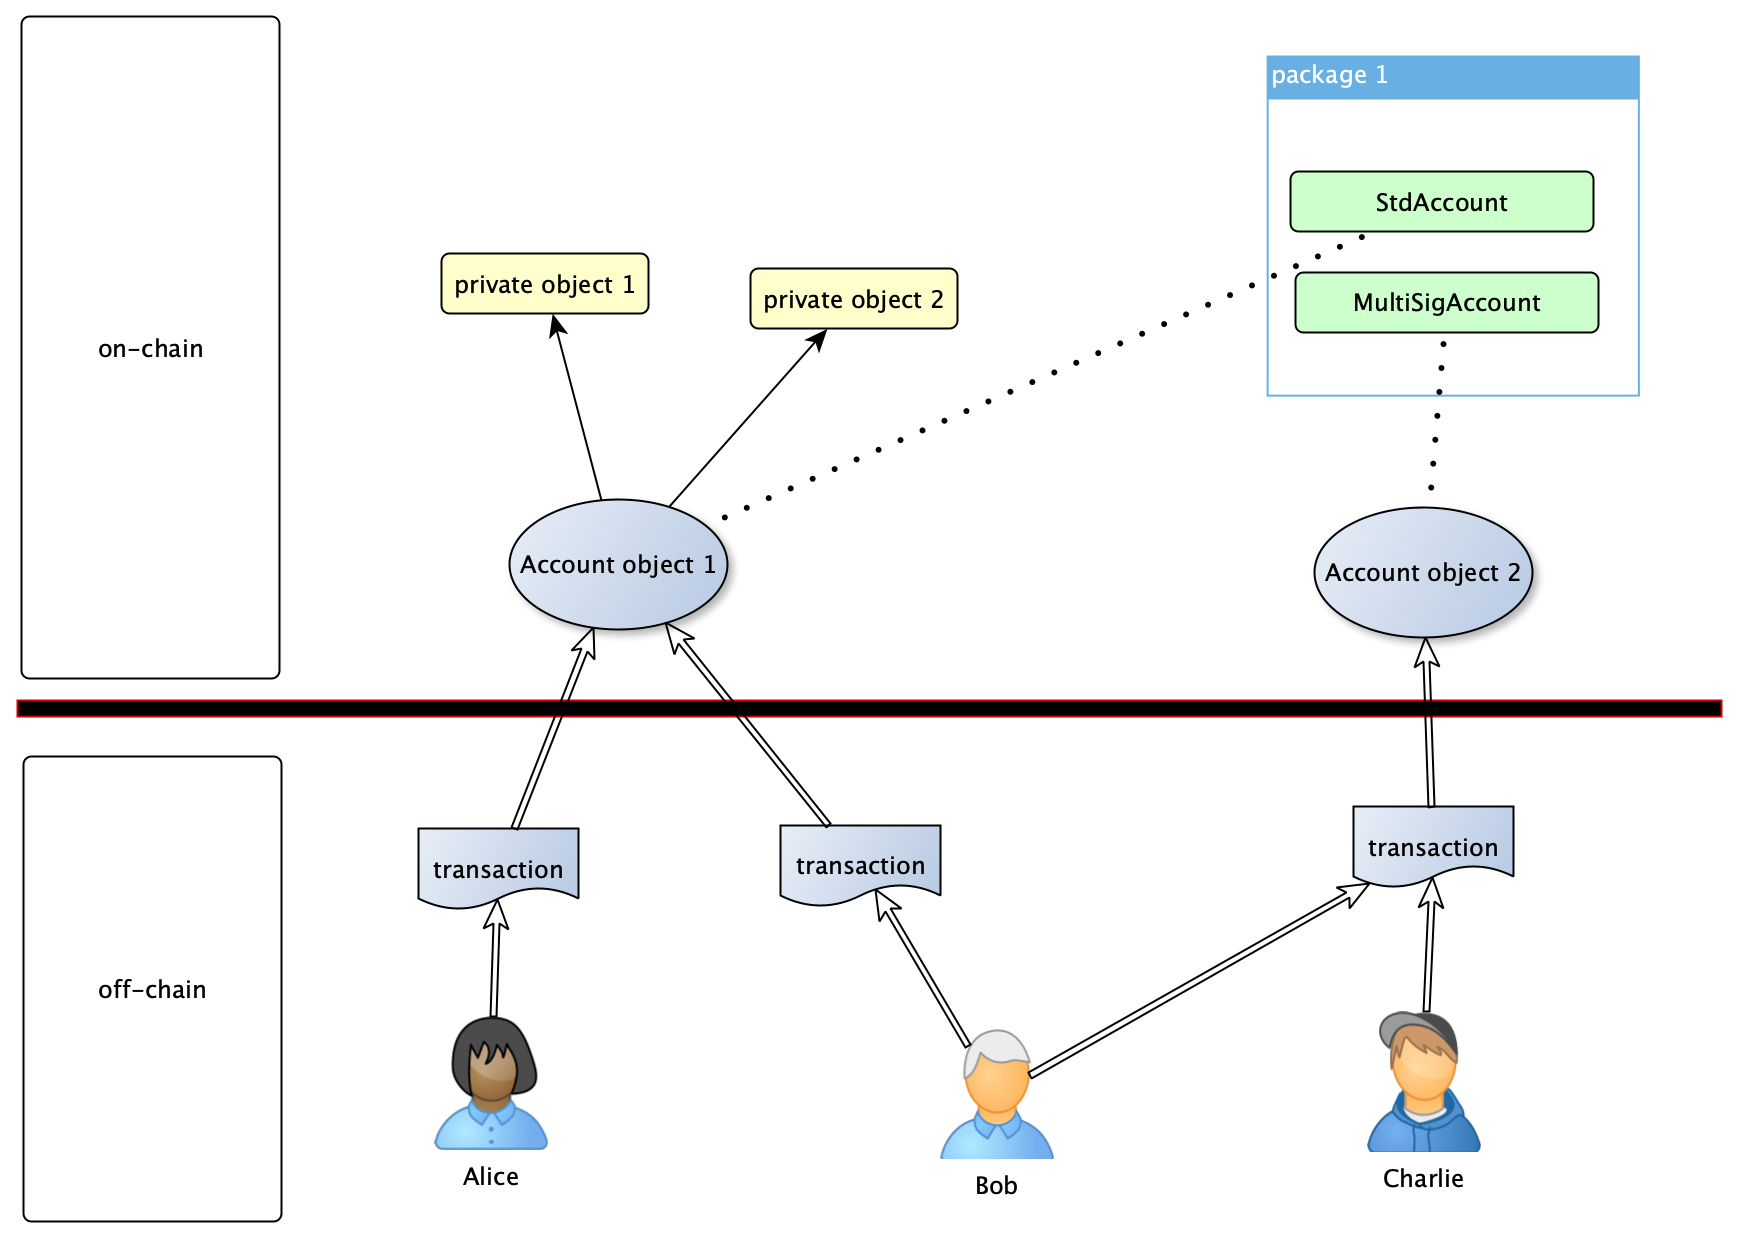
\includegraphics[width=\textwidth]{graphics/account-abstraction.png}
\end{figure}

For an Axi type to be used as a type of account objects it is necessary to implement the \code{Account} interface (caution --- we are still using pseudocode here, go to the appendixes for examples using the actual Axi syntax):

\begin{lstlisting}[language=Rust]
pub trait Account<T: Action> {
  fn verifyTxBatch(&self, batch: TxBatch) -> Option((GasInfo,List<T>));
  fn buildTx(&self, action: T, ledger: Ledger) -> ElaboratedScript
}
\end{lstlisting}

An account object has to implement two methods:

\begin{itemize}
  \item \code{verifyTxBatch()} method is where deserialization and cryptographic verification is to be implemented; it is executed before adding a transaction to the mempool
  \item \code{buildTx()} method is where the execution logic of a transaction is plugged in; it is executed after the consensus orders transactions in a sequence
\end{itemize}

\subsubsection{Account creation and address}

An account is created as any other object: the constructor function from its defining module must be invoked. But, unlike ``normal'' objects, an account object is automatically wrapped in a cell. The address of this cell is generated as a hash of:

\begin{itemize}
  \item constructor method address
  \item arguments passed to the constructor invocation (serialized)
  \item chain-id (explained in the \textbf{Blockchain mechanics} chapter)
\end{itemize}

A new account can be created programmatically --- by an invocation of a suitable native function --- during the execution of any on-chain code. Alternatively, it can be created by executing a special ``self-spawn'' transaction.

\subsubsection{Stubs and self-spawn}

We want Khalani blockchain users to be as sovereign as possible. To achieve this we want every user to have an easy and maximally independent path for creating a blockchain account.

Let's recall first how this works on Ethereum:

\begin{enumerate}
  \item I create a key-pair. This way I can compute the address of my new account.
  \item I arrange some ether (native cryptocurrency) to be transferred to my new account. For this I can ask a friend or just use some external commercial service, where ether can be purchased (such as a crypto exchange, for example Kraken).
  \item I am good to go with sending transactions to my account.
\end{enumerate}

On Khalani, this is a little more complicated, because we have account abstraction. So for an account to be usable, the account object must be created first. For this to happen:

\begin{itemize}
  \item the type of account must be selected first (just the user has to pick one, according to his needs; frequently it will be just the StandardAccount type from the Axi standard library)
  \item corresponding constructor function must be invoked, with all the arguments it requires
\end{itemize}

This can be done all at once, with the support of some dedicated (commercial) service, who in particular will have the means to execute a transaction which will create the account. But there is also an independent path, which the user can execute himself:

\begin{enumerate}
  \item I pick my account type (among the known account types that I deployed in packages on-chain).
  \item According to the cryptographic requirements of the selected account type, I prepare the necessary key pair (or several key pairs).
  \item I compute the account address, which is derived from the constructor address, the serialized parameters and the chain-id.
  \item I arrange some native cryptocurrency to be transferred to my new account. For this I can ask a friend or just use some external commercial service (such as a crypto exchange, for example Kraken). In this phase my account exists on-chain as a so-called \textbf{stub}. This means it has an address and a balance of the native cryptocurrency but the account object is not initialized yet.
  \item I prepare a special transaction called \textbf{self-spawn transaction}. It allows me to provide the details of the account object constructor invocation.
  \item I send the self-spawn transaction to a blockchain node. Upon execution it will replace the stub with a properly initialized account object, retaining all private cells that the stub owned so far (presumably with some native cryptocurrency). The point is that the gas cost for this transaction is covered with my own funds.
  \item I am good to go with sending normal transactions to my account.
\end{enumerate}

Of course the above process is going to be supported by the blockchain tools. The most crucial conclusion here is that thanks to stubs and self-spawn we have both the account abstraction and freedom for the user, who can be as independent as on Ethereum.

\subsection{Delegation}

\subsubsection{Actors on a blockchain}

Before we even delve into the actual delegation problem, we need to discuss the more general problem of ``actors on a blockchain''. In traditional IT, actors are processes (in a single computer) or users (in a security domain) or computers (in a network). But what are actors on a blockchain?

On Ethereum, possible actors are accounts and smart-contracts. Both can own money and both can transfer money.

This situation is a little different in Khalani. On one hand we also have accounts ans services. But technically, both are represented as cells (account cells and shared cells). Hence we end up with the conclusion that in Khalani blockchain actors are just cells. In the Khalani homogenous model, cells serve all purposes.

Therefore when we apply the well-known cryptography convention to use names Alice, Bob, Charlie, Dylan as the actors of a protocol under consideration, we generally think of them as on-chain objects (cells). It is just enough to remember that these objects are flexible enough to represent accounts, services and resources.

\subsubsection{Introducing the delegation problem}

Generally speaking, on a blockchain everything is permission-based. For example, in a basic model of accounts (like on Ethereum) access rights are implied by three rules:

\begin{itemize}
  \item only the transaction sender can transfer ether out of his account
  \item only the smart contract itself can read/write its instance variables
  \item only the smart contract itself can transfer ether out from its balance
\end{itemize}

\textbf{Delegation} is a family of patterns based on a simple common idea:

\begin{quote}

Alice has permission to perform action X. She however has some reasons why she does not really want to perform X by herself. Rather, she wants to ask Bob to perform X on her behalf. For this to be possible, Alice's needs to delegate some of her permissions to Bob.
\end{quote}

Ideally we want the delegation mechanism to be maximally restrictive, so that the scope of Bob's actions while using Alice's permissions is narrow and strictly controlled by Alice. Alice needs this control so that Bob cannot abuse the delegation mechanism against Alice's will.

The lack of a native mechanism of delegation in Ethereum leads to various troubles, generally pushing developers to creating workarounds like this one:

\href{https://eips.ethereum.org/EIPS/eip-2612}{https://eips.ethereum.org/EIPS/eip-2612}

In the meantime, some attempts to introduce general-purpose universal delegation mechanism are underway (ERC-4337 and EIP-7702).

\subsubsection{A motivating example}

Let's look more closely at the example situation we sketched in the Introduction chapter:

\begin{quote}

Say we have Alice (user), Bob, Charlie and Dylan (on-chain services). Bob provides some complicated functionality which involves further interaction with Charlie and Dylan. Alice has no rights to interact with Dylan, so she is forced to use Bob as a privileged intermediary. Charlie recognizes Alice as a user with certain access rights. Bob cannot directly call Charlie because Bob has no rights to do so. Hence Bob would like to interact with Charlie on behalf of Alice
\end{quote}

In the pictures below we use green arrows to denote ``has access'' and red arrows to denote ``access denied''.

So we start with Alice who has a problem:

\begin{figure}[H]
  \centering
  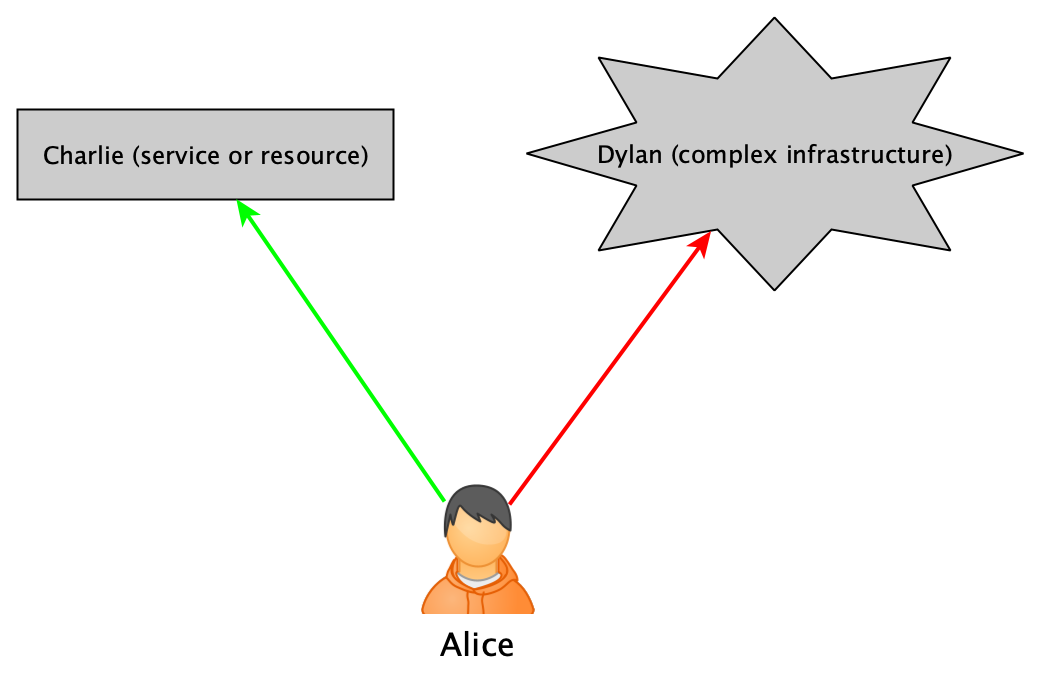
\includegraphics[width=0.5\textwidth]{graphics/delegation-1.png}
\end{figure}

Alice wants to achieve certain business goal. However, for this to happen, Alice would need to contact both Charlie and Dylan. Charlie is a service or resource which Alice has access to. Dylan is a complex or access-restricted infrastructure, which is beyond Alice's reach.

Alice wants to solve her problem. She found a helper service Bob (hence we named it ``a solver''), who can help her with the complicated task of accessing Dylan's infrastructure:

\begin{figure}[H]
  \centering
  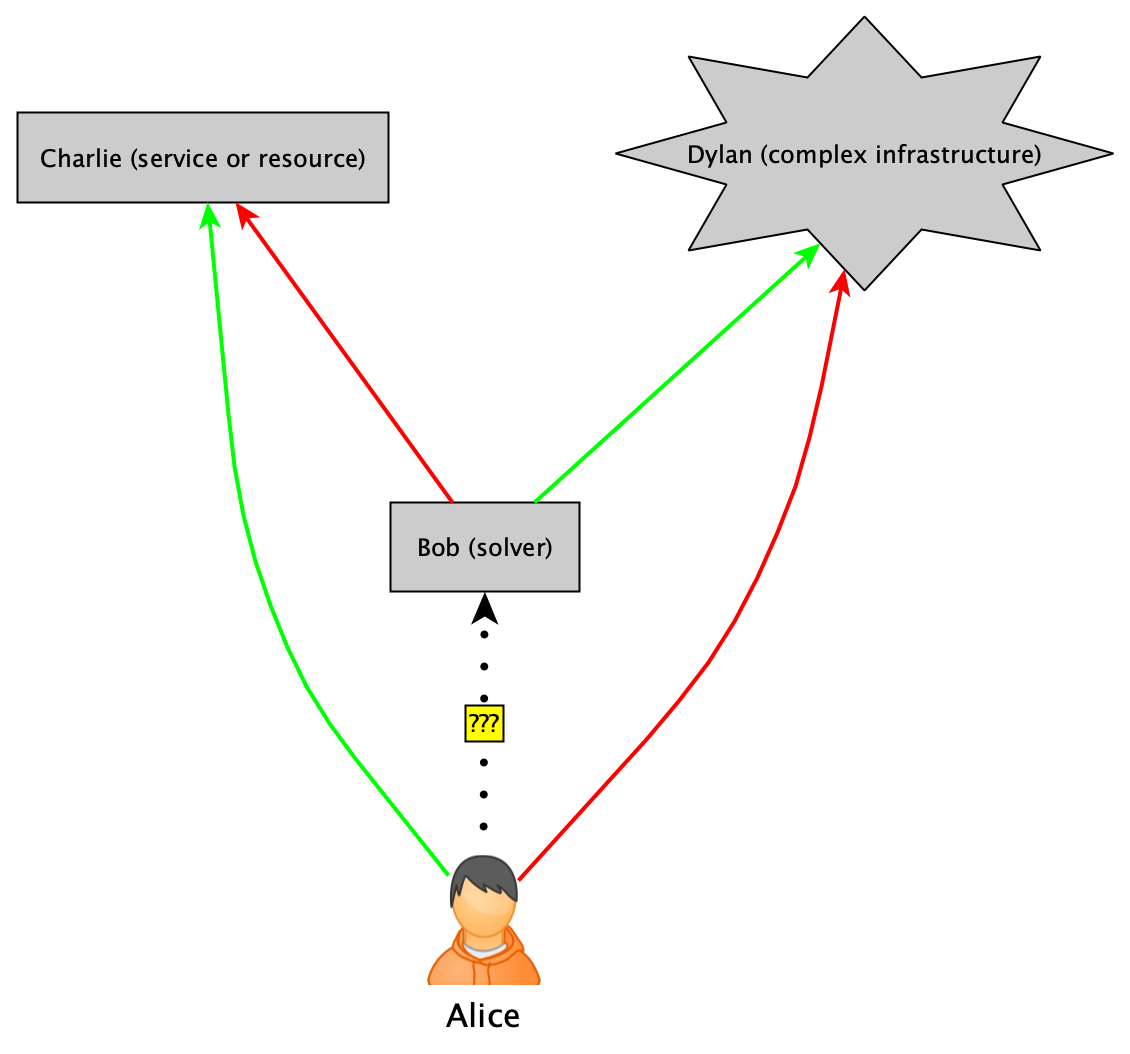
\includegraphics[width=0.5\textwidth]{graphics/delegation-2.png}
\end{figure}

The missing element here is the ability to \textbf{delegate} Alice's access rights. She wants to temporarily lend Bob her ability to access Charlie, so that Bob can solve her problem.

\begin{figure}[H]
  \centering
  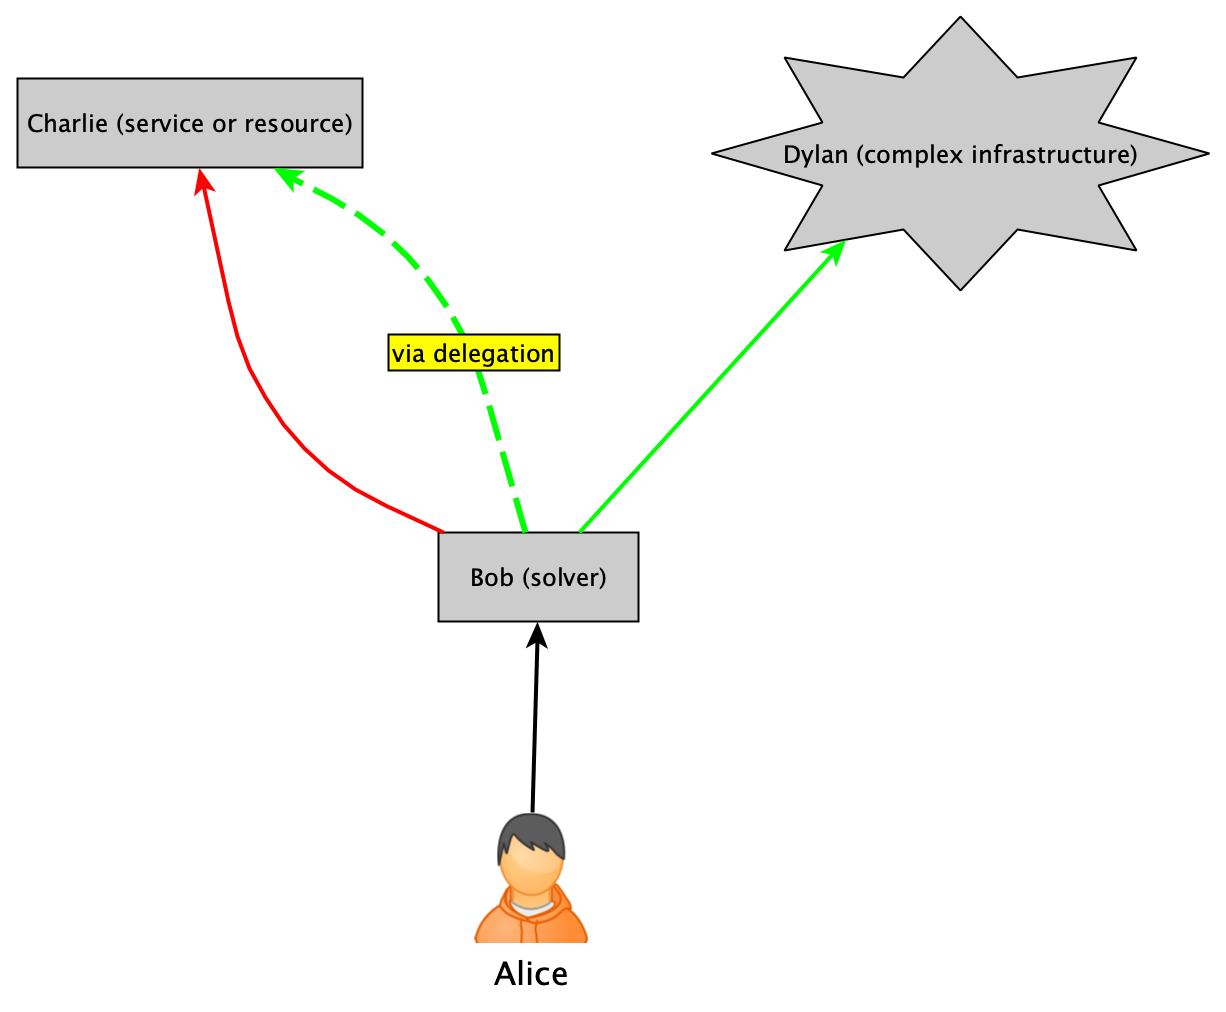
\includegraphics[width=0.5\textwidth]{graphics/delegation-3.png}
\end{figure}

\subsubsection{Delegation in Khalani blockchain}

The delegation mechanism is very powerful and useful, for example it is a crucial element of the intent-based processing infrastructure (which we explain later, in the \textbf{Intents} chapter). At the same time, any such mechanism is extremely dangerous, because by its very nature it bypasses access-rights limitations, hence malicious players can utilize this as a universal fraud tool.

In Khalani, we attempt to get the best of both worlds: maximal safety and maximal flexibility. Therefore, we do not follow the Ethereum's delegation strategy. Instead, our delegation model is based on a variant of the capability pattern. We allow Alice to form a so-called ``speculative handle'' to represent her rights to access Charlie. Alice can pass such a handle to Bob so as to execute the delegation of privileges. However, this delegation is non-exclusive (i.e. can be given to several solvers) and it can also be revoked. That being said, the mechanism is still under research and we have not decided what will be its final form.

\subsection{Pub-sub, timers and gas reserve}

\subsubsection{Pub-sub on-chain}

Publish-subscribe is a well established programming pattern:

\href{https://en.wikipedia.org/wiki/Publish–subscribe_pattern}{https://en.wikipedia.org/wiki/Publish--subscribe\_pattern}

In most mainstream blockchains every smart contract can emit events, but these events are observable only by off-chain agents. Such a version of pub-sub is of course useful, but it has severe limitations. For example, if used for the solvers' reputation system (for the context what are solvers' reputation systems and why they are needed, go to the \textbf{Intents} chapter) then the off-chain relayer is needed so as to pass events to an on-chain reputation registry. This relayer then happens to become a centralization point, undermining trust. This is especially troublesome given the fact that the solvers' reputation system is all about establishing the trust levels for solvers.

The escape from such circular problems is simple when a blockchain supports on-chain pub-sub mechanics:

\begin{itemize}
  \item every smart contract can announce events
  \item every smart contract can subscribe/unsubscribe to events
  \item subscription is just handler registration
  \item when an event is emitted, all the registered handlers are invoked
\end{itemize}

From the developer's perspective, this can be captured as follows:

\begin{lstlisting}[language=Rust]
type EventHandler<T> = fn(String, data: T);

pub trait EventEmitter<T> {
  fn subscribe(&self, event_symbol: String, handler: EventHandler<T>);
  fn subscribe_one_off(&self, event_symbol: String, handler: EventHandler<T>);
  fn unsubscribe(&self, event_symbol: String);
  fn emit(&self, event_symbol: String, data: T);
}
\end{lstlisting}

However the semantics of on-chain events is more tricky than it is for traditional Ethereum-like event systems with off-chain observers only. The new problem here is: who pays gas for the handler's execution? We discuss this problem in the next chapter.

\subsubsection{Gas reserve}

Obviously we cannot charge the event emitter --- this would be against the very idea of events: emitter only announces things and does not expect any penalty for this.

Therefore, it seems logical it should be the subscriber who pays the gas. Now it becomes clear why Ethereum does not support on-chain pub-sub: the desired gas charging semantics would fundamentally break the gas model of Ethereum.

Without pub-sub, the payment model is simple: the whole call tree gas cost is covered by the balance of the sender account:

\begin{figure}[H]
  \centering
  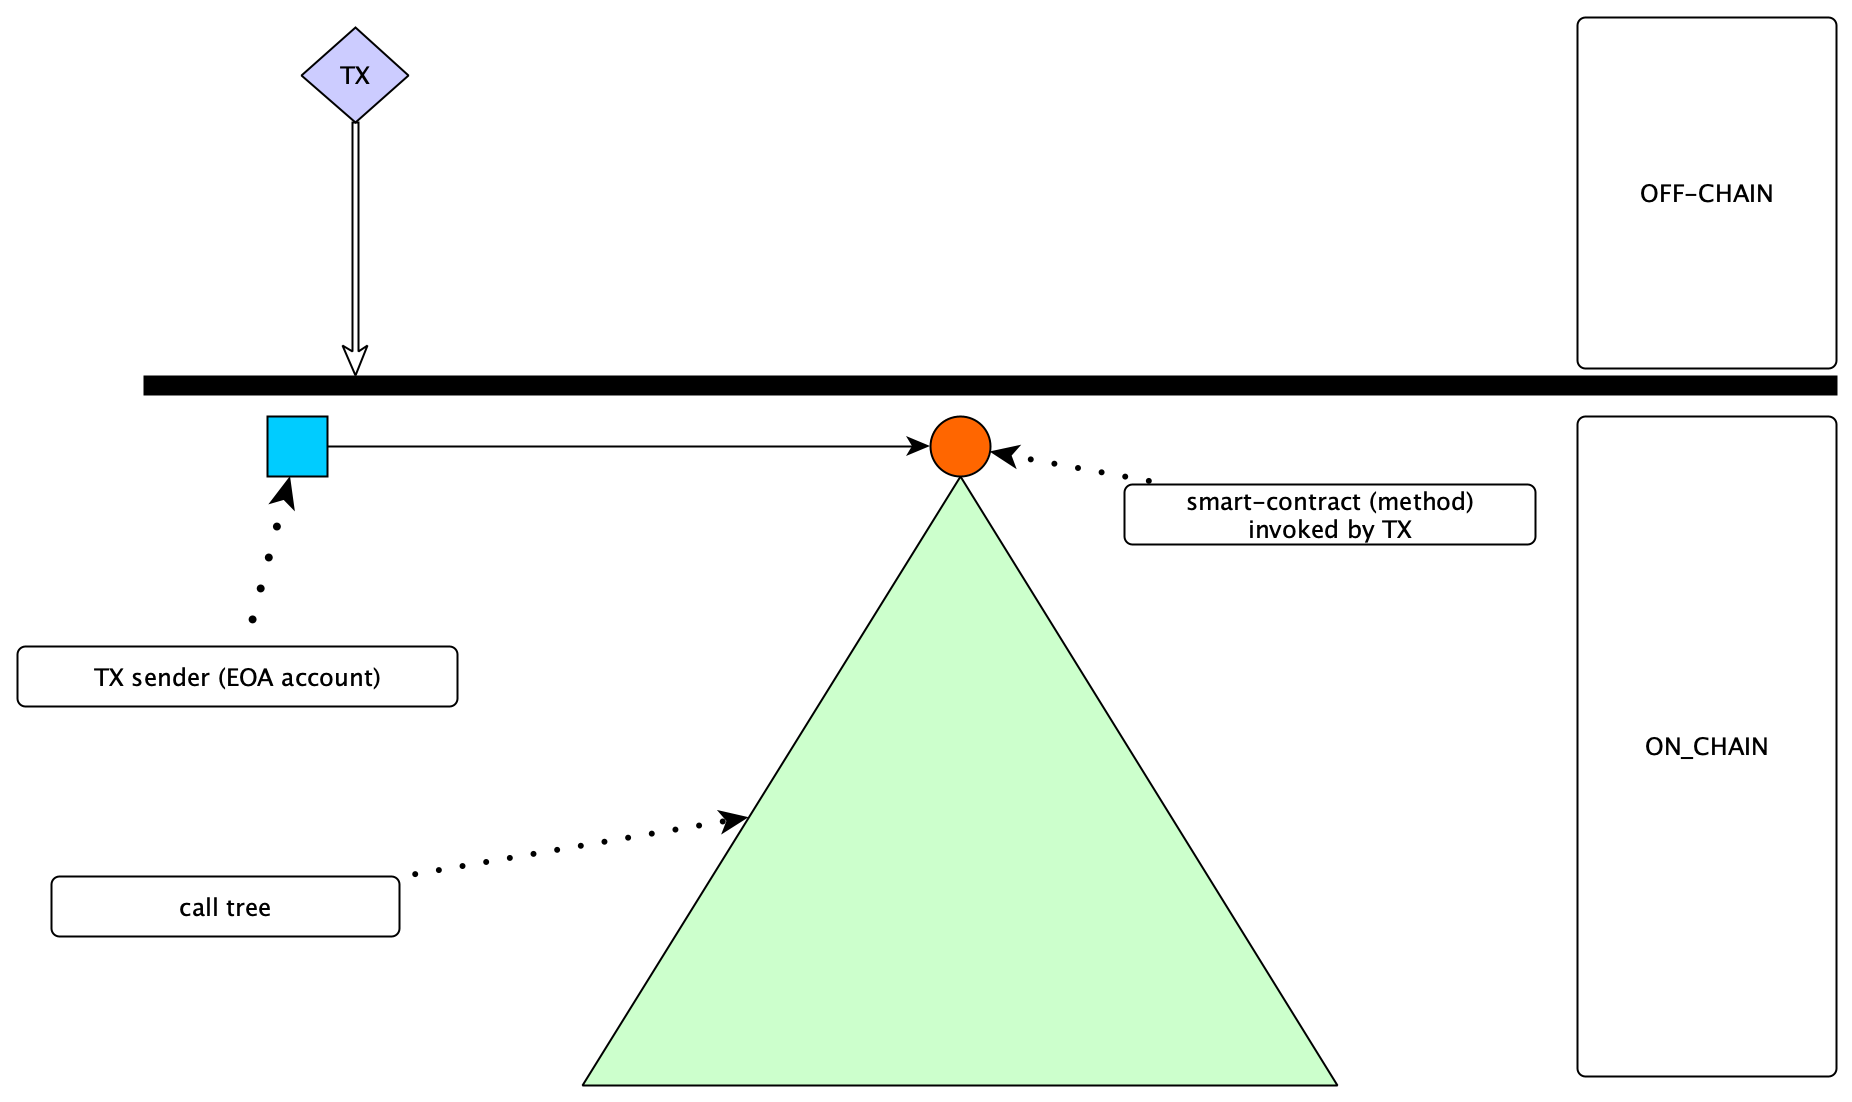
\includegraphics[width=\textwidth]{graphics/gas-cost-without-pub-sub.png}
\end{figure}

With pub-sub present, the situation gets more tricky. The invocation of an event handler is not really a ``call'', because it is the pub-sub machinery doing this call. Hence every handler invocation spawns a separate call tree.

\begin{figure}[H]
  \centering
  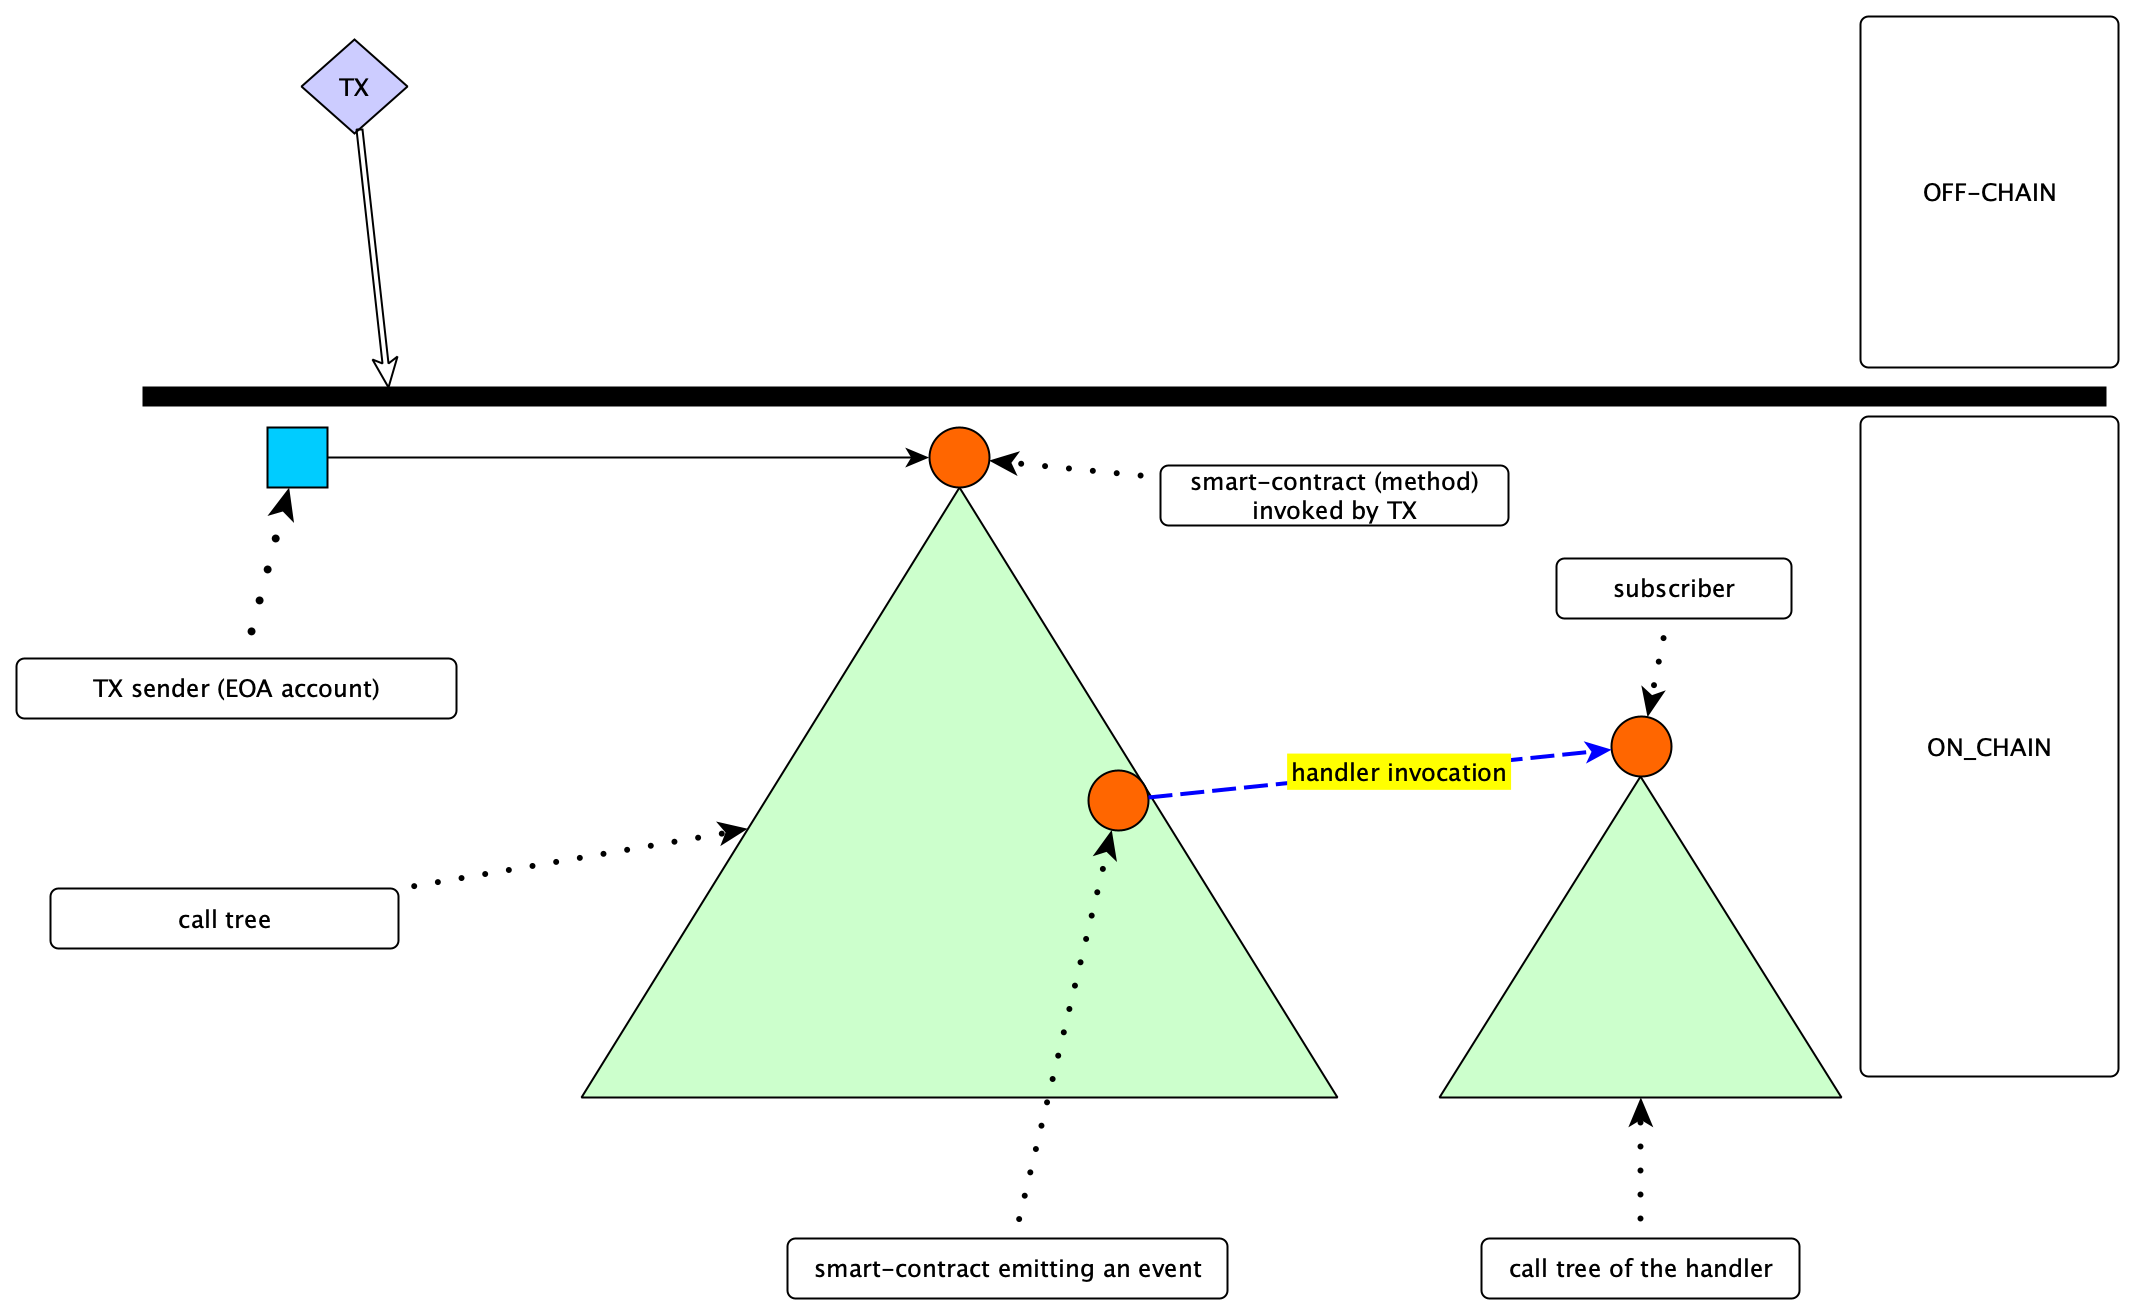
\includegraphics[width=\textwidth]{graphics/gas-costs-with-pub-sub.png}
\end{figure}

We previously said that it should be the subscriber who pays the gas for the handler's execution. But even this is tricky. It can be:

\begin{itemize}
  \item the subscriber --- understood as the smart-contract that registered the handler
  \item the subscriber --- the sender of the transaction who invoked handler registration
\end{itemize}

Both approaches turn out to be somewhat disappointing. Big part of the problem is that gas prices are fluctuating over time. What should the system do if the gas cost of the handler execution is not sufficiently covered? The only reasonable option is to roll back the whole handler invocation. Unfortunately, such an approach makes the whole pub-sub abstraction too non-deterministic to be useful.

A safer deterministic design can be obtained if we combine the following rules:

\begin{itemize}
  \item ``best effort'' subscriptions and ``guaranteed'' subscriptions are distinguished
  \item ``guaranteed'' subscriptions are one-off (i.e. get cancelled after one handler call)
  \item ``guaranteed'' subscriptions are covered with gas reserve (see below)
  \item the handler registered during a guaranteed subscription must follow the static gas regime (see below)
  \item explicit \textbf{gas reserve} is maintained by every smart contract (or gas is turned into a separate cryptocurrency)
  \item static gas estimation is supported (for sufficiently limited sublanguage of the native smart-contract language)
\end{itemize}

\subsubsection{On-chain timers}

Timers are almost like pub-sub, but it is the clock who triggers the invocation of a handler. Of course, for this to be possible, the concept of ``clock'' must be somehow available on-chain. In the simplest approach, the time is represented as the height of the current block.

From the developer's perspective this can be captured as follows:

\begin{lstlisting}[language=Rust]
fn register_timer(timepoint: BlockchainTime, handler: EventHandler<T>): Timer;
fn cancel_timer(timer: Timer);
\end{lstlisting}

The question of who pays for timer handler's execution leads to similar considerations as it was in the case of pub-sub. We analyze this problem in depth in the next chapter.

\subsubsection{Transactional approach to pub-sub and timers}

The traditional approach to covering gas cost is: the execution cost of the whole call tree is paid by the transaction sender. However --- as we argued above --- this model breaks down when calling handlers: someone else is to pay for the handler. It leads to an interesting question: if the call tree of a transaction A invoked a handler B (effectively another call tree) and during the execution of B's call tree the corresponding gas/cryptocurrency reserve has been exhausted --- what should happen? Of course the execution of call tree B has to stop immediately. But the state of the blockchain cannot stay inconsistent, so we need to do a rollback. But because an event emitter must be shielded from any errors during the execution of handlers, it leads to the conclusion that we need to roll back call tree B only, while A's call tree will stay intact.

The simplest way to achieve this isolation and to retain the original gas semantics is to assume that handler invocation is executed as a separate transaction.

In other words, on a blockchain with on-chain pub-sub we would have three types of transactions:

\begin{itemize}
  \item external tx
  \item internal tx (pub-sub handler invocation)
  \item internal tx (timer's handler invocation)
\end{itemize}

External transactions are sent to nodes by clients. Internal transactions are added by the VM on-the-fly during the execution. The only remaining question is the ordering. The outcome of the consensus protocol is the linear ordering of blocks, and linear ordering of (external) transactions inside of blocks.

Our idea of handlers execution leads to the following behavior: when the block is executed, necessary internal transactions will be created and inserted into the original sequence of external transactions. This process can be illustrated as the following tree:

\begin{figure}[H]
  \centering
  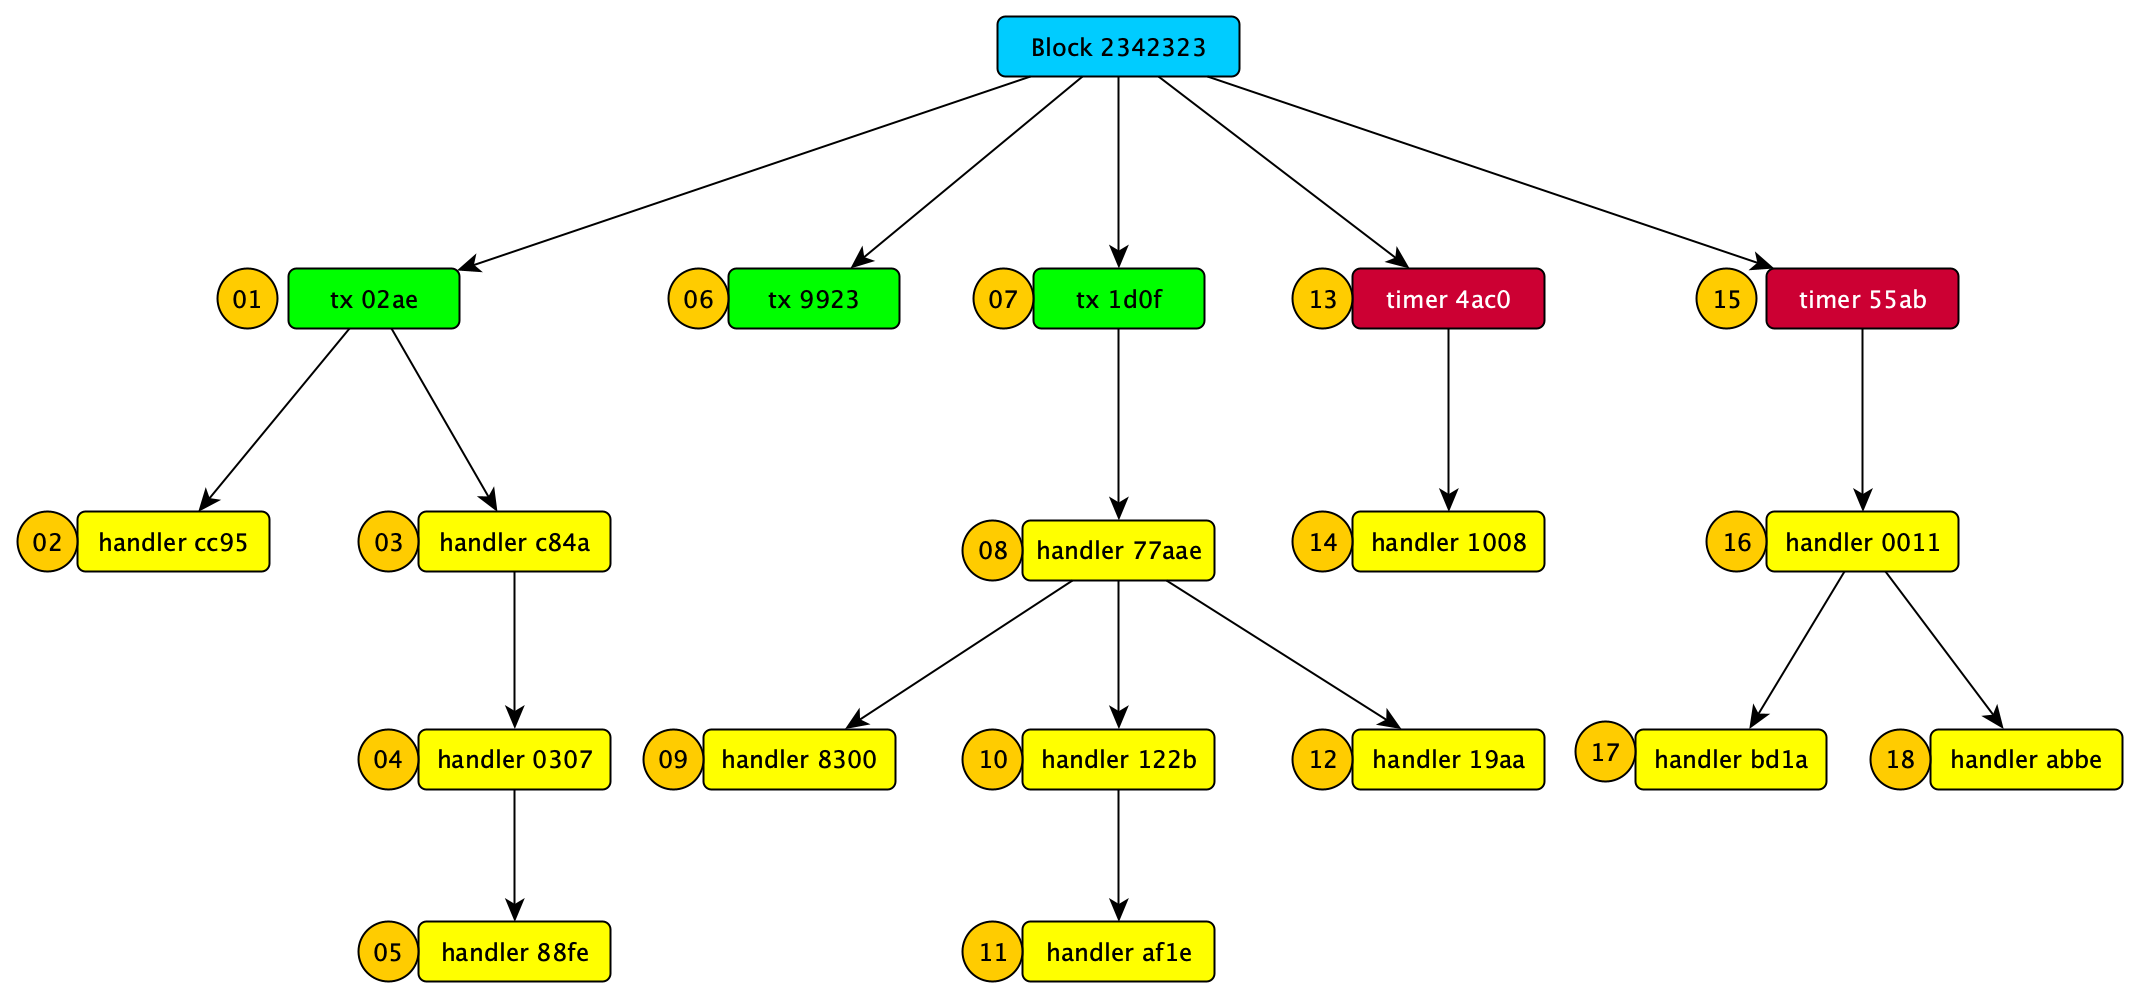
\includegraphics[width=\textwidth]{graphics/handlers-invocation-sequence-simplified.png}
\end{figure}

\begin{enumerate}
  \item Colors:
  \begin{enumerate}
    \item green --- external transactions (ordered by the consensus protocol)
    \item yellow --- pub-sub handlers invocations
    \item red --- timers handlers invocations
  \end{enumerate}
  \item While executing any transaction, the VM accumulates handler invocations launched by event emitters. Every such handler invocation will then be executed in a separate (internal) transaction.
  \item Because any on-chain code can emit events, this means that any transaction (internal or external) can spawn new transactions by emitting events. This leads to a tree where nodes are transactions and edges are handler invocations. Because the whole block has the same blockchain time, timer handlers are placed at the end of a block (after all the external transactions). Their ordering should be implied by the ordering of respective subscriptions.
  \item Ordering of child nodes is implied by the order of handler invocations:
  \begin{enumerate}
    \item for different \code{emit()} invocations, the order of resulting internal transactions follows from the ordering of emit() calls (on-chain code is executed sequentially)
    \item for a single \code{emit()} invocation, the order of resulting internal transactions follows from the order of subscriptions
  \end{enumerate}
  \item Ordering of all transactions in a block is achieved as the variant of depth-first-search traversal of the tree, where every parent node is visited before its child nodes.
  \item This algorithm ensures the following properties:
  \begin{enumerate}
    \item The ordering of external transactions as achieved by the consensus protocol is never changed.
    \item If (internal or external) transaction T1 precedes transaction T2, then all event handlers spawned by T1 will be executed before T2.
    \item Gas for every transaction (internal or external) is charged separately.
    \item Execution of event handlers (including any errors) does not influence the execution of the transaction that emitted events which spawned these handlers. In particular, rollback of a handler transaction will not influence the transaction where the corresponding event originated.
  \end{enumerate}
\end{enumerate}

\subsubsection{Our approach}

The exact way timers, pub-sub and gas reserve will be operated at the Axi level is under active research. Nevertheless, we want all three mechanisms to be available.

Most likely we will not introduce gas as a separate cryptocurrency, because this may lead to the creation of a massive gas trading market, which in turn could undermine the reason for gas existence --- gas is there to achieve supply-demand balance around the processing capacity of the blockchain nodes network. Therefore we are leaning towards a more limited gas reserve semantics, where cells of kind ``account'' and ``shared'' can accumulate private, non-transferable gas reserve for their own use only.

The gas price to be paid when buying gas for the reserve is P\% bigger than the gas price of the current block. The fluctuation of the parameter P would then be subject to decentralized management by validators voting or it will be controlled by some in-protocol mathematical formula depending on the total value of gas burned in the last N blocks vs current total amount of gas reserve.

The way gas reserve is used is going to be integrated into Axi declaratively: a function that is annotated with a suitable \code{using-gas-reserve} marker will always be executed by utilizing the gas reserve of the shared object or the account object (depending on the declaring module).

Also, because we want provability and this involves proving behaviors that depend on events, the static-gas sublanguage of Axi will be delineated. The VM will be able to compute the gas cost of a function written in the static-gas sublanguage of Axi by static analysis. Static-gas sublanguage can then be used to implement any handler that is part of a ``critical'' functionality, so that a correct gas reserve can be allocated upfront.

\subsection{Intents}

\subsubsection{Intent-driven processing}

\textbf{Intent-driven processing} is a novel movement in the blockchain industry that postulates a new form of interaction with blockchains, where instead of sending a transaction (or a collection of transactions), a user only specifies the boundary conditions for a desired outcome. A specification of such boundary conditions is otherwise known as an \textbf{intent}. The act of bringing the blockchain state to the shape defined by an intent is referred to as \textbf{filling this intent}. Software agents that fill intents are referred to as \textbf{solvers}.

An intent-based ecosystem is then formed, where:

\begin{itemize}
  \item customers publish intents
  \item solvers observe incoming intents and engage when they can see a business opportunity
  \item matching between customers and solvers is done either directly via the native intents support or via a suitable ``intents market''
\end{itemize}

Intent-driven processing can be seen as a far-reaching generalization of the decentralized exchanges ecosystem, where intents generalize trading orders and intent markets generalize DEXes.

\subsubsection{Intent-based processing vocabulary}

\begin{itemize}
  \item \textbf{Intent:} a specification of the desired effect/state of the blockchain; an intent is created by a user and usually has a form of a digitally signed document
  \item \textbf{Filling an intent:} materializing the desired outcome (as specified by an intent); this is the work that a solver does
  \item \textbf{Intentbook:} registry of intents (usually stored on-chain)
  \item \textbf{Solver:} a software agent capable of filling (some) intents
  \item \textbf{Solving:} overall activities done by a solver (includes participating in counterparty selection protocols, filling, settlement and off-chain activities)
  \item \textbf{Counterparty selection:} a process of deciding which solver will be given the privilege to fill a given intent
  \item \textbf{Selected solver:} the solver that got selected via the counterparty selection process
  \item \textbf{Settlement:} the final processing of an intent where the successful filling is confirmed and the reward is paid to the selected solver
  \item \textbf{Reward:} a certain amount of money (paid in on-chain assets) that the selected solver gets for filling an intent
  \item \textbf{Fiasco:} the situation where the winning solver failed to fill an intent before the specified deadline
  \item \textbf{Rollback:} the process of returning the funds to the intent's creator (if any funds were actually locked) after a fiasco
\end{itemize}

\subsubsection{Intent markets}

We do not want to hardcode a fixed intent-based ecosystem into the Khalani blockchain. Rather, we believe the right way to approach the problem is to ensure that a blockchain provides a sufficiently versatile toolbox of mechanisms needed for building such ecosystems.

We anticipate that the future of intents is going to be primarily driven by the concept of \textbf{intent markets}, for which we introduce the new term ``i-market''. An i-market is a far-reaching generalization of a Dex:

\bigskip
\begin{tabularx}{\textwidth}{|l|X|}
\hline
\textbf{Dex concept} & \textbf{Corresponding concept in i-markets} \\
\hline
order & intent \\
\hline
orderbook & intentbook \\
\hline
order execution & filling \\
\hline
order type (limit order, market order, stop order...) & intent type \\
\hline
\end{tabularx}
\bigskip

In particular, every Dex is an i-market.

It is the responsibility of an i-market to define:

\begin{itemize}
  \item representation of intents
  \item types of intents it can handle
\end{itemize}

Some i-markets can just provide intent filling service by themselves. Other i-markets can delegate solving work to dedicated third-party services (solvers), hence becoming broker-like services, with the primary responsibility of connecting intent originators (customers) and intent fillers (solvers).

In the most extensible form an i-market can be:

\begin{itemize}
  \item solver-pluggable (i.e. allowing any solver to join)
  \item intent-type-extensible (i.e. allowing new intent types to be defined and used)
\end{itemize}

For the intent-type extensibility we anticipate that the crucial abstraction --- \textbf{mandarin} --- is needed. A mandarin is a service-like cell that orchestrates the processing of a single intent. In other words, a mandarin is a self-executing trading agreement, established by parties involved in a trade. The mandarin lifecycle corresponds to the execution process of the corresponding trade.

Typically, the involved parties that use a mandarin for orchestrating a trade will be:

\begin{itemize}
  \item intent creator (i.e. ``customer'')
  \item solver (i.e. ``service provider'')
\end{itemize}

In parallel with the adoption of intent-based trading we should observe an increase of well-known mandarin types deployed on-chain (with their specifications and proofs). There will be dedicated mandarin types for an extensive list of trading situations, for example:

\begin{itemize}
  \item simple token swaps
  \item cross-chain token transfers
  \item NFT item swaps
  \item conditional swaps
  \item asset-lending agreements
  \item various derivatives (such as options)
  \item conditional investing
\end{itemize}

But this is just the beginning. Over time, off-chain service providers will find their way to use intent-capable blockchains as decentralized integrators of off-chain services. Currently we have a large collection of such integrators, just operating as centralized services, for example:

\begin{itemize}
  \item Amazon (integrator of online shops)
  \item \href{http://Booking.com}{Booking.com} (integrator of hotel services)
  \item Airbnb (integrator of short-term apartment renting services)
  \item Uber (integrator of people transportation services)
\end{itemize}

Over time, intent-based markets will appear as a viable alternative to such service integrators. This in turn will go in parallel with completely new mandarin types --- corresponding to apartment renting intents or transportation intents. Ultimately, thanks to the intent-based infrastructure, blockchains will become perfect platforms for integration of off-chain services (because there is no provider lock-in and provider bias --- unavoidable in the case of centralized integrators).

An implementation of a fully-pluggable i-market has to address the following topics:

\begin{itemize}
  \item maintaining the database of intents (i.e. the intentbook)
  \item counterparty selection (possibly several strategies)
  \item mandarin creation
  \item solver's backend (so that solvers can connect to the market and be informed about incoming intents)
  \item reputation infrastructure for solvers
\end{itemize}

\subsubsection{Mandarins}

As we stated before, a Dex is also an example of an i-market. But in a Dex all intent types (traditionally they call them ``order types'') are just hardcoded. There is a handful of them implemented inside of a Dex and this is it.

In the upcoming intent-based processing wave the whole point is in building i-markets that are not confined by a hardcoded list of intent types. Rather, we want such an i-market to support any intent types. So we want pluggable intent types.

This means an i-market has to define a suitable format of an ``intent-type'' plugin. In Khalani we actually suggest how this can be accomplished. We call this ``the mandarin pattern''.

\begin{figure}[H]
  \centering
  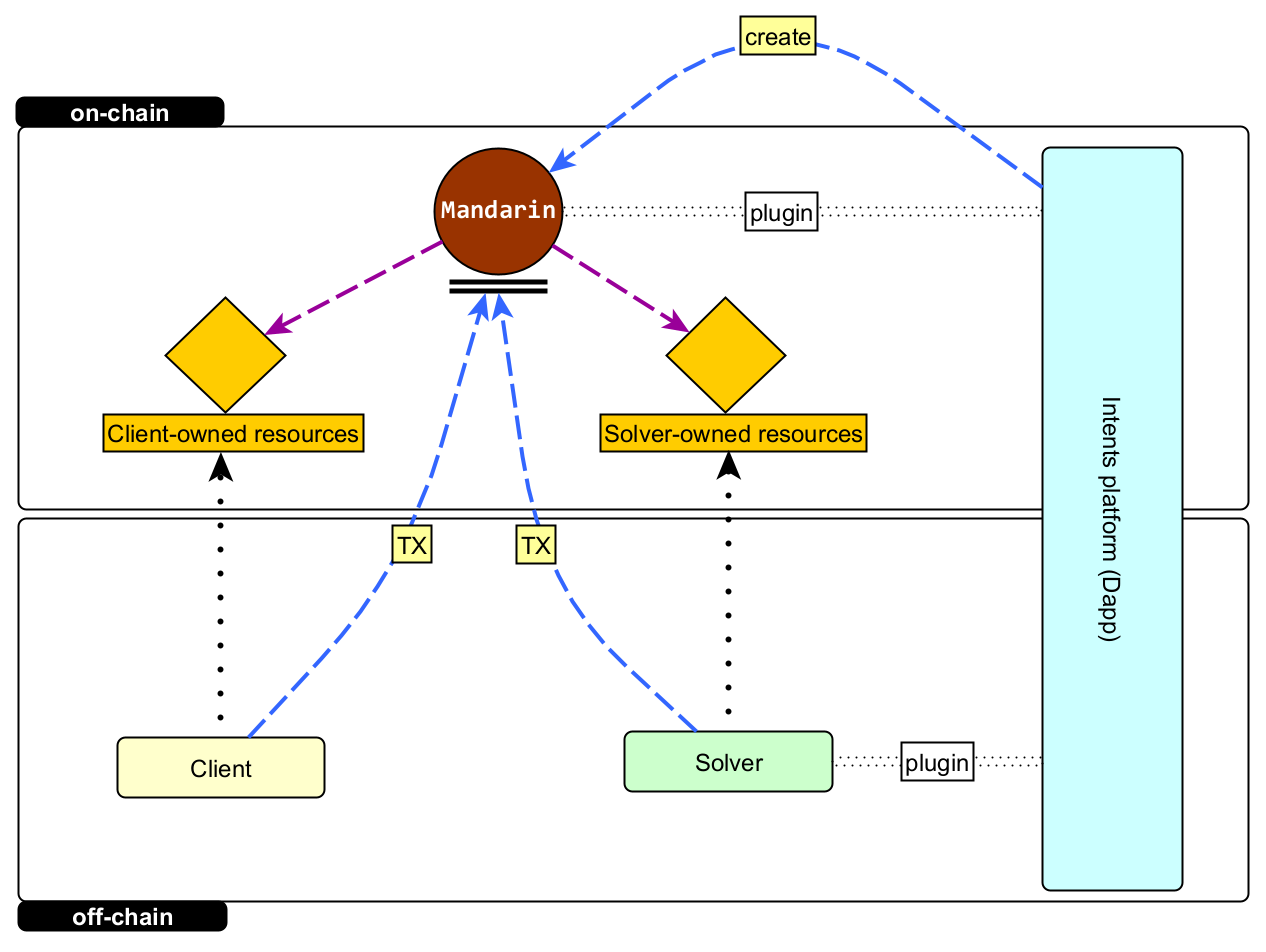
\includegraphics[width=\textwidth]{graphics/mandarin-interaction.png}
\end{figure}

There are two layers of this pattern:

\begin{itemize}
  \item \textbf{mandarin type} --- this is the code that implements one kind of intent (i.e. one trading pattern)
  \item \textbf{mandarin object (instance)} --- the cell typed with a mandarin type; it orchestrates the execution of one intent
\end{itemize}

It is not necessary, but probably convenient, for mandarin objects (we just call them ``mandarins'') to be created by the i-market.

A mandarin must know the participants of the trade (typically these participants will be: a customer and a solver). Its lifecycle is bound to orchestrating the execution of the trade it was created for. After the execution is completed (successfully or with a failure), a mandarin dies.

Typically, a mandarin will use delegation to perform actions on behalf of the trade participants. It will also use pub-sub to announce its lifecycle events, so that the corresponding i-market can observe mandarins it has created (for the purpose of solvers' reputation management).

A mandarin can be seen as a far-reaching generalization of the escrow concept. From this perspective the mandarin pattern is all about allowing programmable escrows that are capable of taking actions by themselves and that are observable via on-chain events.

\subsection{Code as asset}

We want the authors of good on-chain code to be financially rewarded. Therefore Khalani blockchain supports two complementary mechanisms:

\begin{itemize}
  \item every package has an owner (which is an account); an owner can be changed, in other words, on-chain trading of packages is possible
  \item the current owner of a package gets financial profits (``royalties'') every time code from this package is executed
\end{itemize}

\subsubsection{How royalties work}

Whenever the VM executes Axi code, it computes gas. Gas measures the amount of computation and storage effort that the blockchain needed to invest into the execution. Every piece of code is declared in a package. The royalty is computed as a constant fraction \code{P} of the overall gas spent executing code from this package.

Additionally, whenever a new package gets deployed, a constant fraction \code{Q} of its deployment gas cost is equally distributed as royalty to all packages it (transitively) imports.

Once distributed to packages, the royalty gas is immediately converted back to the native cryptocurrency (more precisely, the gas units --- distributed as royalties --- are then used to proportionally pay the transaction gas fee to all relevant package owners).

\subsubsection{Trading of packages}

Packages can be traded. But because this is public code, for transparency (and safety of code owners) the only way a package can be traded is via a public and open on-chain auction. The mechanics of code-trading auctions will be implemented as an on-chain service, sealed into the blockchain at Genesis.

It works like this:

\begin{itemize}
  \item An owner of the package invokes a special function that starts the auction process. This is the last thing he can do, because the auction cannot be revoked. As a result, an auction mandarin will be created.
  \item The duration of the auction is a protocol constant and is expressed as blockchain time (i.e. number of blocks in consensus). We imagine the auction should be approximately one month long.
  \item Bidding happens via invoking a \code{bid()} method of the auction mandarin. Bidding involves the actual transfer of the money (always in the form of Khalani native cryptocurrency). The money offered by the last bidder money gets locked in the auction mandarin. The bidding releases previously locked money (returns it back to the previous bidder).
  \item Whoever wins the auction, will take over the ownership of the package. The money paid by the winner is automatically transferred to the previous owner of the package.
  \item If nobody participated in the auction, the ownership of the package stays unchanged.
\end{itemize}

\subsubsection{Donation to the public domain}

Packages can be ``donated to the public domain''. Specifically, the owner may relinquish his ownership at any time. This will cause that royalties for using the donated package will no longer be charged. A package donated to the public domain will stay as public domain forever, i.e. the donation is irreversible.

In particular the Axi standard library will be deployed to the Khalani blockchain at Genesis in a form of a collection of packages. These packages will be deliberately donated to the public domain since day one.

After a fixed period following deployment, every package automatically gets donated to the public domain. This fixed time is a protocol parameter. We envision it to be set to 15 years.

\subsubsection{Gas usage statistics}

Because royalties are paid as a fraction of the actually burned gas, package authors earn more if their code is less gas efficient. This is of course not a good correlation, because it looks like a violation of incentive compatibility. However, the situation is actually not that bad because the on-chain code in Khalani forms an open market. If there is a way to gas-optimize a popular package, someone may actually implement a gas-optimized version, deploy it and advertise its existence to the community, so that people will migrate their code to use the more efficient version.

However, for this to work in practice, two conditions must be met:

\begin{enumerate}
  \item Developers need an easy way to ensure that the new package actually does the same job as the old one.
  \item Developers need an objective way of comparing the average gas efficiency between packages.
\end{enumerate}

We provide both:

\begin{itemize}
  \item (1) is addressed by the strong type system, in particular by traits and concepts.
  \item (2) is addressed by per-function average gas statistics (collected only for package public functions), which the VM will accumulate and publish on-chain, so they are objective and accessible from the block explorer (statistics will be updated on every transaction and confirmed by consensus).
\end{itemize}

\subsection{Blockchain mechanics}

\subsubsection{Gas}

Gas is computed by the VM. We consider separating gas into computation gas and storage gas, but this aspect is still under research.

Every transaction declares:

\begin{itemize}
  \item max gas price the sender is willing to pay
  \item gas limit for this transaction
\end{itemize}

Within a single block, the protocol sets a fixed gas price equal to lowest gas price offered by transactions included in the block. Therefore, all transactions in a single block pay the same gas price. We hope this approach will help stabilize gas prices and prevent unjustified gas price rising.

\subsubsection{Transaction structure and execution}

Transactions have the following structure:

\begin{lstlisting}[language=Rust]
struct TransactionMetadata {
  protocol_version: u16,
  account_address: Address,
  nonce: u256,
  target_epoch: Epoch,
  expiration: BlockchainTime,
  ancestors: Vec<TransactionHash>
}

struct NormalTransaction {
  metadata: TransactionMetadata,
  payload: Bytes,
  signature: Bytes
}

struct SelfSpawnTransaction {
  metadata: TransactionMetadata,
  gas_fee_sources: Vec<Address>,
  constructor_call: FunctionCall
}

struct GasInfo {
  gas_limit: Gas,
  gas_price: GasPrice,
  gas_fee_sources: Vec<Address>
}

pub trait Account {
	type Action;
  fn verifyTxBatch(&self, batch: TxBatch) -> Option<(GasInfo,List<T>)>;
  fn buildTx(&self, action: Action, ledger: &mut Ledger) -> ElaboratedScript;
}
\end{lstlisting}

There are two types of transactions:

\begin{itemize}
  \item normal
  \item self-spawn
\end{itemize}

A normal transaction is really a ``batch of actions'', which will get executed sequentially but atomically. It is as if the user can glue together a list of transactions, so that either all of them will get executed correctly, or the whole batch will be reverted.

The payload of a normal transaction is a byte-array. It is the account object who:

\begin{itemize}
  \item parses the payload and validates the signature (this happens upon the admission to the mempool)
  \item executes the transaction --- by preparing the Axi script to be executed
\end{itemize}

The way transactions are built allows for extreme flexibility: a transaction build at the client side can actually include a script wrote in Axi. We just enforce that in such a case the type-checking phase happens at the client side, so that the ``elaborated'' source code in AST form is sent over (not just bare source code). This way we shield the blockchain from DoS attacks based on exponentially-hard type-checking attacks.

\subsubsection{Replay attacks prevention}

A replay attack is a known hacking technique, where a previously signed correct transaction is reused by a hacker. There are two possible scenarios of such a reuse:

\begin{itemize}
  \item A fixed transaction is sent over and over again (to the same blockchain node) --- this could be used as a DoS attack or for malicious draining of the resources of the victim account.
  \item The transaction is sent to another chain based on the same protocol (like reusing a Testnet transaction on Mainnet).
\end{itemize}

In Khalani we put in place mechanisms to prevent both scenarios:

\begin{enumerate}
  \item \textbf{TX nonce}: A transaction contains the \code{nonce} field. The sender puts a randomly generated 256-bit value there. This is supposed to enforce that every transaction is unique. For performance reasons, nodes are unable to check this uniqueness globally, but they do not have to --- because it is enough to keep the transaction hashes index for the last two epochs. This way uniqueness of transactions within the epoch can be enforced. Because every transaction also has the \code{target\_epoch} field, this makes it impossible to use old transactions for replay attacks.
  \item \textbf{Chain-id:} The genesis block id (which is its 256-bit hash) serves as the identifier of the chain. This chain-id is then added as a ``salt'' in the transaction hash value calculation (which is then used for tx signature). This way every transaction is valid only in the context of a single chain. Other chains will reject such a transaction as having an invalid signature.
\end{enumerate}

\subsubsection{Blocks and consensus}

We have not decided yet which consensus protocol will be used in the Khalani blockchain. Most likely this will be a variant of proof-of-stake, which takes into account the native concurrency of the UTXO model.

The UTXO model is a hypergraph, where transactions are hyper-edges. The computational dependencies between transactions have the structure of a partial order. What the consensus protocol has to do is to achieve Byzantine agreement across blockchain nodes with regard to this partial order. An example of such a protocol is Mysticeti:

\href{https://sui.io/mysticeti}{https://sui.io/mysticeti}

\newpage

\begin{appendices}

% Display "Appendix <letter>: ..." as the appendix title.
\makeatletter
\renewcommand{\@seccntformat}[1]{%
  \@ifundefined{#1name}{}{\csname #1name\endcsname~}%
  \csname the#1\endcsname: }
\makeatother

\section{Overview of Axi}

Axi (pronounced ``Axee'') is the smart contract language of Khalani. It is a purely functional programming language with a strong, static, linear type system and support for formal reasoning about programs in classical higher-order logic. Among mainstream programming languages, it is most similar to Haskell (in spirit) and OCaml (syntactically). It was also heavily inspired by proof assistants based on type theory, like Coq, Lean and Agda.

In this appendix we will have a brief, not too technical look at the philosophy and language features of Axi.

\subsection{Philosophy}

Axi's architecture is unique in that the language is split into two strictly separate layers: the programming layer and the logic layer.

\textbf{The Programming Layer} of Axi is a purely functional language based on \href{https://en.wikipedia.org/wiki/System_F#System_F%CF%89}{System \(F_{\omega}\)} (the higher-order polymorphic lambda calculus) with a quantitative, resource-aware type system (linear, affine, relevant and unrestricted types).

Axi aims to make programming pleasant and comprehending smart contract code easy, while providing essential guarantees to all on-chain code:

\begin{itemize}
  \item \textbf{Type safety}. Well-typed programs can't go wrong, i.e. they can't crash, can't perform nonsensical operations like adding a number and a string, nor can they result in any other runtime type error.
  \item \textbf{Memory safety}. Well-typed programs can't result in memory errors, like writing to a random memory location, nor can they have memory leaks.
  \item \textbf{Resource safety}. Well-typed programs can't create, delete or copy resources unless it is allowed by the resource type's interface, nor can they access resources stored on the ledger unless authorized by the resource's owner.
\end{itemize}

\textbf{The Logic Layer} of Axi is a language for reasoning about Axi programs in classical higher-order logic. It allows expressing arbitrarily complex mathematical properties, thus allowing programmers to give precise specifications of the business logic and behaviour of their programs. These specifications can then be proved for all possible inputs. Proofs provide guarantees much more powerful than those of the type system alone, while being as credible and trustworthy as the type system. The use of the logic layer is entirely optional, i.e. programmers are never forced to engage with any part of it. However, we plan to encourage them to make use of logic by making smart contracts' competition for reputation be partially based on the formal guarantees they provide.

\textbf{Strict separation}. In Axi, logic can reason about programs, but programs cannot manipulate logical entities, like theorems or proofs, at runtime. This one-way interaction keeps the language relatively simple, while still making it possible to express almost all functional programming idioms and all possible mathematical properties and their proofs.

\textbf{Guarantees about guarantees}. We not only want Axi to provide strong guarantees about its programs, but we also want to provide strong guarantees about Axi itself. We plan to use the Coq proof assistant to formally verify significant portions of Axi's metatheory, including the aforementioned properties of type and resource safety, as well as the consistency of Axi's logic. We are also considering formal verification of the reference implementation of Axi. The goal of these efforts is to ensure that the guarantees that Axi provides are trustworthy and will stay so forever, as long as the consensus protocol is followed.

\subsection{Language features}

In this section we will take a closer look at Axi's language features.

\subsubsection{The Programming Layer}

Axi is, at its core, a purely functional programming language. It therefore supports all the usual features of such languages:

\begin{itemize}
  \item \textbf{Purity and immutability}. In Axi, all values are pure and immutable -- they cannot be null, cannot throw exceptions and once created, they cannot be changed. Variables are also immutable and cannot be changed once asssigned a value (although we allow name shadowing). This facilitates reasoning about and comprehending code, thus rendering Axi smart contracts transparent and auditable.
  \item \textbf{First-class, higher-order and anonymous functions}. Functions are first class citizens. They can be passed as arguments to other functions, returned from other functions as results and created on the fly. Axi encourages a programming style in which data is processed by pipelines built from basic building blocks like mapping, reducing, filtering and so on.
  \item \textbf{Algebraic data types and pattern-matching}.
  Axi makes it easy to model the problem domain with disjoint unions and define functions by pattern matching. This allows programmers to write code for which simple invariants are encoded directly in the shape of the types, decluttering it from clunky boolean flags and cascades of conditional expressions.
  \item \textbf{Strong static type system}. Axi's type system makes it easy to work with high-level abstractions, like merkle trees or state machines, instead of low-level primitives, like integers or byte arrays. It is lightweight, not placing too many demands on the programmer, but still catches the most egregious errors -- it can easily protect programmers from confusing with each other such objects as an integer, a string, an address, a transaction hash, a token amount and a cryptographic secret.
  \item \textbf{Traits}. Axi supports traits inspired by Haskell's type classes (but named after Rust's traits). A trait is a way of representing an interface satisfied by a type. The definition of a trait consists of a bunch of declarations of constants and functions. The programmer can make a type an \textit{instance} of a trait by implementing the trait's constants and functions for this type. Traits allow expressing familiar concepts, like functors and monads.
  \item \textbf{Polymorphism}. Axi's type system features parametric polymorphism (also known as ``generics''). Together with traits, these features make it easy to implement data structures and functions that work for all types that support a certain behaviour, for example a hash map that works for all types of ERC-20-compliant tokens bridged from an external blockchain.
\end{itemize}

\textbf{Quantitative typing}. The standard features of purely functional programming is not everything that Axi has to offer. The killer feature, as far as the programming layer is concerned, are \emph{quantitative types}. Quantitative types control the variable usage discipline: which values are allowed to be copied and which are allowed to be left unused. This aspect of Axi's type system was inspired by linear logic and its cousin, quantitative type theory, and is an improvement upon an analogous feature of the type system of Move, the programming language of the Sui and Aptos blockchains.

In an Axi program, every variable is assigned its \textit{quantity}, which can be either: zero, one, at most one, at least one, unrestricted. The variable's quantity determines how many times it can be used in the program, with too many or too few uses resulting in a type error. For example, the typical variable holding an NFT will have a quantity of one, forcing the program to do something with the NFT before it terminates: maybe send the NFT to the transactor, maybe trade it for something else and handle that something else properly according to its quantity, or maybe send it to somebody as a gift. What the program cannot do in such a situation is forget the NFT and do nothing with it, effectively making it ``lost'' in the guts of the chain. It also cannot copy the NFT and have two instead of just the original one.

To make the programmers' lives easier, every type is also assigned its ``default'' quantity. Every variable will be assigned the default quantity of its type unless the programmer decides otherwise. An important piece of terminology: a type whose default quantity is unrestricted is called a \textit{data type}, whereas a type whose default quantity is either one, at least one or at most one, is called a \textit{resource type}. There are no types whose default quantity is zero. Elements of data types are called data, whereas elements of resource types are called resources.

\subsubsection{The Logic Layer}

Axi's logic layer consists of typed classical higher-order logic with equality whose domains of discourse are the types from the programming layer. More precisely, this means the logic has:

\begin{itemize}
  \item \textbf{Propositional connectives and constants}. Standard propositional connectives ($\Longrightarrow$, $\land$, $\lor$, $\Longleftrightarrow$, $\sim$) and constants ($\top$, $\bot$) can be used to build up complex propositions from simpler ones.
  \item \textbf{Quantification over terms and types}. Axi supports universal and existential quantification. We can quantify over terms of a given type ($\forall x : A, \dots$) as well as over types themselves ($\forall A : \texttt{Type}, \dots$), no matter whether we're dealing with data, resources or programs.
  \item \textbf{Higher-order quantification}. We can also quantify over logical entities like propositions ($\forall P : \texttt{Prop}, \dots$), predicates ($\forall P : A \rightarrow \texttt{Prop}, \dots$), relations ($\forall R : A \rightarrow A \rightarrow \texttt{Prop}, \dots$), logical connectives ($\forall C : \texttt{Prop} \rightarrow \texttt{Prop} \rightarrow \texttt{Prop}, \dots$) or even quantifiers themselves ($\forall Q : (A \rightarrow \texttt{Prop}) \rightarrow \texttt{Prop}, \dots$). This ability of logic to talk not only about the underlying programming language, but also about itself, gives it great expressive power and allows it to make use of all of mathematics when reasoning about the behaviour of programs.
  \item \textbf{Equality}. The built-in equality relation ($=$) makes it possible to precisely reason about programs' input-output behaviour.
  \item \textbf{Concepts -- traits in logic}. Last but not least, Axi's logic can not only talk and reason about the traits from the programming layer, but it also introduces the richer and more powerful construct called \textit{concepts}. Concepts extend traits with specifications, i.e. properties expected to be true of the trait's constants and functions. When implementing a concept, the programmer must also provide proofs of the specifications. As a result, concepts let programmers precisely define what is expected of trait implementations.
\end{itemize}

Proving is carried out in a proof language based on the Curry-Howard correspondence: proofs of implications and universal quantifiers are like functions, proofs of existential quantifiers and conjunctions are like pairs, proofs of disjunctions are like disjoint union constructors, etc. Negation and biconditional are handled as in intuitionistic logic -- instead of being primitives, negation ($\sim P$) is a shorthand for an implication into falsehood ($P \implies \bot$), whereas biconditional ($P \iff Q$) is a shorthand for a conjunction of two implications ($(P \implies Q) \land (Q \implies P)$). The principle of \textit{proof by contradiction}, which allows to prove ($(\sim P \implies \bot) \implies P$) for any proposition $P$, makes the logic classical and thus intimately familiar to all mathematicians.

Equality is handled as in Martin-Löf Type Theory -- proved by reflexivity and eliminated with the so-called J rule, which is a principle that allows to substitute equals for equals in the remaining part of the proof. Because proofs are hard to write using these primitives, Axi provides a convenient feature called \textit{chaining}, which allows reasoning with long chains of equations by writing down and justifying each step separately, similarly to how equality is usually handled with pen and paper. Besides equality, this feature also supports implications, biconditionals and other transitive relations.

One novel feature that distinguishes our proof language is that the proofs can be presented in two styles: either in a \textit{proof term style}, similar to how proofs look in Agda and Idris (as well as Coq's and Lean's manually written proof terms), or in a \textit{tactic style}, similar to how proofs usually look in Coq or Lean. The difference between Axi and languages that also support both styles, like Coq and Lean, is that in these languages each style is its own separate proof language, whereas in Axi there is a single proof language which, thanks to a clever parser, can be formatted either like terms or like tactics. This feature will make it easier to accomodate computer scientists and mathematicians familiar with either of the aforementioned languages.


\newpage

\section{Code examples}

In this section, we will see some code examples that demonstrate how Axi works in practice. Note that Axi is not implemented yet, so the code examples are only an approximation of what we intend to achieve, rather than a demonstration of an existing language.

\begin{example}{A simple program --- list functions}

\lstinputlisting{listings/FunProg.axi}

\end{example}

The above example demonstrates the basics of Axi programming. On lines 1-3 we define an algebraic data type called \code{List}. The type is parameterized by a type \code{A} and has two constructors: \code{nil} is the empty list and \code{cons h t} is the list with head \code{h} and tail \code{t}. Both \code{:\ Type} annotations on line 1 are necessary, because we need to indicate that both \code{A} and \code{List A} are unrestricted types, as opposed to linear, affine or relevant types (we will see these in later examples).

On lines 5-8 we define a function called \code{app} which concatenates two lists. It takes three arguments: a type \code{A} and two lists \code{l1} and \code{l2} of type \code{List A}, and returns a result of type \code{List A}. The type argument means that the function is polymorphic. It is also marked with the symbol \code{@}, which means it is an \textit{implicit} argument, i.e. when calling the function it can be omitted and will get automatically inferred. The body of the function is simple: we pattern match on the argument \code{l1}. If it's \code{nil}, we return \code{l2}. If it's of the form \code{cons h t}, we return a list whose head is \code{h} and whose tail is computed by the recursive call \code{app t l2}.

On lines 10-12 we define another function, called \code{map}, which applies a function \code{f} to every element of a list. This time, however, we use an abbreviated syntax. The two type arguments \code{@A} and \code{@B} are marked as implicit, but we don't need to write the \code{:\ Type} annotations, which get inferred automatically. The argument \code{f} and its type are written out in full. Then, instead of taking another argument, we say the function returns a function of type \code{List A -> List B}. Because we omit the equality sign, what follows in the next two lines is a definition by pattern matching on the output function's \code{List A} argument.

\begin{example}{Quantitative typing}

\lstinputlisting{listings/CopyDrop.axi}

\end{example}

The above example demonstrates how the type system enforces resource discipline. We will define the type \code{KhalaniCoin} and the function \code{coinMerge} in the next example. For now it only matters that \code{KhalaniCoin} is a linear type, i.e. \code{KhalaniCoin\ :\ Type1}.

First, on line 3, we try to define a function called \code{coinForgery}. It takes an argument of type \code{KhalaniCoin} called \code{x} and returns a \code{KhalaniCoin} by calling the function \code{coinMerge} with both its arguments being \code{x}. Now, \code{KhalaniCoin} is a linear type, i.e. by default variables of this type must be used exactly once. Because \code{x} is of type \code{KhalaniCoin} and nothing indicates otherwise, this means that the function \code{coinForgery} must use \code{x} exactly once. However, it uses it twice when calling \code{coinMerge}, which is a type error.

This error is caught by the type checker, which complains that \code{x} was used too many times. The error message also hints at some possible solutions: use \code{x} less (the only solution for ordinary programmers) or redefine the type \code{KhalaniCoin} to allow duplicate uses (this solution is only available to the type's implementer). The fact that the type system was able to catch this error is crucial, because if the function \code{coinForgery} passed the type checker, it would allow programmers to create unbounded amounts of \code{KhalaniCoin}, causing hyperinflation, which most likely was not the intention of this type's creator.

The second function, called \code{coinBlackhole}, takes an argument \code{x} of type \code{KhalaniCoin} and returns \code{()}, which is the only value of type \code{Unit}, which is the type with only one element. The fact that \code{Unit} is the return type indicates that the function's result ``doesn't matter''. Because the type of \code{x} is linear, \code{coinBlackhole} must use \code{x} exactly once. However, it doesn't use it at all, which is a type error.

This error is caught by the type checker, which complains that \code{x} was not used. Similarly to the previous error message, two hints are offered: use \code{x} or make the type \code{KhalaniCoin} affine so that it allows zero or one usages (with the latter solution being available only to the type's creator). The fact that this error was caught by the type system is very important, because the creator of \code{KhalaniCoin} did not intend for values of this type to be deletable.

\begin{example}{\code{Coin} trait}

\lstinputlisting{listings/Trait.axi}

\end{example}

The above example shows the definition of the \code{Coin} trait, which could be one way of capturing the commonalities of user-defined coins. Then we implement the type \code{KhalaniCoin} from the previous example and demonstrate how to make it an instance of the \code{Coin} trait.

On lines 1-5 we define the trait \code{Coin}. It takes a parameter \code{A :\ Type1}, which is a linear type that represents the type of coins. The trait has one constant and three functions. \code{coinZero} represents a coin with denomination zero (but we will prefer the word ``amount'' instead of denomination). \code{coinMerge} merges two coins. \code{coinSplit} splits one coin into two, with its first argument being the amount of its first output and the second output being the change; there is also the possibility of failure if the amount asked is too large, indicated by \code{Option} wrapping the first output's type. \code{coinAmount} is perhaps the most mysterious --- it returns the amount of the coin, but also a new coin. This is a pattern that we will see many times. If it returned just the amount, calling \code{coinAmount} would destroy the coin, because it must be used exactly once (because its type is linear), and checking the amount counts as a single use! Therefore, \code{coinAmount} must not only return the amount, but also a ``new'' coin, which we expect to be the same as the ``old'' coin (but this property is not guaranteed; later we will see how to guarantee it using logic).

On lines 7-8 we implement the type \code{KhalaniCoin}. It is a record type with a single field \code{amount} which is a natural number (i.e. a non-negative number which can be arbitrarily large). \code{KhalaniCoin} is a linear type, because we marked it with the annotation \code{:\ Type1}. Note that this is the case even though its only field, \code{amount}, is of type \code{Nat}, which is not a linear type. In other words, the programmer is free to turn data into resources if he so wishes (although he may not freely turn resources into data).

On lines 10-29 we implement the trait \code{Coin} for the type \code{KhalaniCoin}. Note that we don't need to implement the trait's constants and functions in the same order they appear in the trait definition. On lines 11-12 we implement \code{coinZero} --- it is a record (of type \code{KhalaniCoin}) whose \code{amount} field is \code{0}.

On lines 14-15 we implement \code{coinMerge}. It takes two arguments of type \code{KhalaniCoin} and returns a \code{KhalaniCoin} which is a record whose \code{amount} field is the sum of \code{amount}s of its arguments.

On lines 17-19 we implement \code{coinAmount}. It takes an argument \code{c} of type \code{KhalaniCoin} and returns a tuple whose first component is a natural number and whose second component is a \code{KhalaniCoin}. First, on line 18, we consume the coin \code{c} by peeking at its \code{amount} field, which then gets named \code{n}. On line 19, we build the return tuple --- the first component is just \code{n}, whereas the second component is a record whose \code{amount} field is \code{n}. Note that the latter is exactly the same as the initial coin \code{c}, but we cannot directly return \code{c} as the second component, because \code{c} must be used exactly once and we have already used it when checking its \code{amount}.

Last but not least, on lines 21-29 we implement \code{coinSplit}. It takes two arguments, \code{askedAmount} of type \code{Nat} and \code{c} of type \code{KhalaniCoin}. First, on line 23, we consume \code{c} to check its amount and store it in \code{n}. Then, on line 24, we check if \code{n} is large enough for the split to succeed. If it does, on lines 25-27 we return a tuple whose first component is a coin whose amount is the \code{askedAmount} (wrapped in \code{some} to indicate success) and whose second component is a coin whose amount is \code{n} minus the \code{askedAmount} that went to the other coin. If \code{n} is not large enough, we return a tuple whose first component is \code{none} (to indicate failure) and whose second component is a coin whose amount is \code{n}, i.e. a coin that is the same as the original coin \code{c}.

\begin{example}{A simple proof}

\lstinputlisting{listings/SimpleProof.axi}

\end{example}

The above example shows a simple theorem and its proof. On line 1 we see the theorem's name, \code{app-assoc}, which is a mnemonic for ``(list) append is associative''. Its statement, on lines 2-3, reads as follows: for all types \code{A} and for all \code{l1}, \code{l2}, \code{l3} which are of type \code{List\ A}, the list \code{app\ (app\ l1\ l2)\ l3} is equal to the list \code{app\ l1\ (app\ l2\ l3)}. Note that here the symbol \code{@} marks the three arguments as \textit{explicit}, whereas its absence for \code{A} marks this type argument as implicit --- opposite to the convention used in the programming layer. These details, however, won't be very important for us now.

The proof is on lines 4-17. At any point in the proof, Axi keeps track of all the \textit{goals} that need to be solved to finish the current proof and also of the \textit{context} of these goals, which is the list of all local objects and assumptions we can use in the proof. When we start the proof with the keyword \code{proof}, we start with a single goal that is the same as the theorem statement. The code on line 5 can be read as ``let \code{A} be any type and let \code{l1} be any value of type \code{List A}''. At this point the goal becomes \code{forall (l2 l3 :\ List A), app (app l1 l2) l3 === app l1 (app l2 l3)}. On line 6 we indicate that the rest of the proof proceeds by induction on the list \code{l1}. The induction has two cases, \code{nil} and \code{cons}, corresponding to the two \code{List} constructors. This means that we now have two (sub)goals, one for each case.

On line 7 we indicate the start of the (sub)proof for the first goal, i.e. the \code{nil} case. At this point our current goal is \code{forall (l2 l3 :\ List A), app (app nil l2) l3 === app nil (app l2 l3)}, because \code{l1} was replaced with \code{nil}, and after line 8 it is \code{app (app nil l2) l3 === app nil (app l2 l3)}. Note that this information is not shown in the code --- displaying the goal and context to the programmer will be handled by language tools like IDE plugins. We finish the first subgoal on line 9. \code{refl}, which is short for ``reflexivity'', indicates that this equation holds trivially, just by computing the result on both sides.

On line 10 we indicate the start of the (sub)proof for the second goal, i.e. the \code{cons} case. On the same line we bind the arguments of \code{cons}, which we name \code{h} and \code{t}. We also get hold of our induction hypothesis for \code{t}, which we name \code{IH}. After line 11, the current goal is \code{app (app (cons h t) l2) l3 === app (cons h t) (app l2 l3)}, as \code{l1} was replaced with \code{cons h t}.

On lines 12-16, we use \textit{chaining} to finish the goal. It works like this: on line 13, after the equality symbol \code{===}, we write the left-hand side of the current goal (which must be an equation), which in our case is \code{app (app (cons h t) l2) l3} (line 13). Then, on subsequent lines, we write out what this expression is equal to (again, after \code{===}) and provide justifications (i.e. proofs) for why this is the case (after the keyword \code{by}). In our case, on line 14 we indicate that our goal's left-hand side is equal to \code{cons h (app (app t l2) l3)}, but we omit the justification for this. We could have written \code{by refl}, but this is the most trivial justification possible, so Axi guesses this is what we mean when we omit a justification. Then, on line 15, we indicate that it is equal to \code{cons h (app t (app l2 l3))}, justifying it with \code{by rewrite IH}, i.e. we are making use of our induction hypothesis. This justification is crucial and cannot be omitted, because Axi cannot infer it on its own. Finally, on line 16, we indicate that our expression is equal to the right-hand side of our goal, again omitting the justification, because it is trivial. All in all, the entire chaining proves that \code{app (app (cons h t) l2) l3} is equal to \code{app (cons h t) (app l2 l3)}, which is exactly what our goal was. Thus, the proof is finished, which we indicate on line 17 with the keyword \code{qed}.

\begin{example}{\code{LawfulCoin} concept}

\lstinputlisting{listings/Concept.axi}

\end{example}

The above example shows the definition of a \textit{concept} called \code{LawfulCoin} and its implementation for \code{KhalaniCoin}. \code{LawfulCoin} takes as a parameter one linear type \code{A}, which moreover must implement the \code{Coin} trait. This is what it means for the \code{LawfulCoin} concept to \textit{extend} the \code{Coin} trait. Note this distinction: the trait and its implementation are part of the programming layer, whereas the concept and its implementation are part of the logic layer.

On lines 2-3, we define a function \code{coinAmount'} that is part of the \code{LawfulCoin} concept. This is a feature we have not mentioned before: both traits and concepts, besides declarations, can also contain (auxiliary) definitions. In our case, we need the function \code{coinAmount'} to avoid using the much more cumbersome \code{coinAmount} when stating the properties that lawful coins should satisfy. \code{coinAmount'} takes an argument of type \code{A} (which we think of as a coin, because it has the \code{Coin} trait) and returns only the first output of \code{coinAmount}, while ignoring its second output.

It might seem that \code{coinAmount'} ignoring the coin returned by \code{coinAmount} is a type error (zero uses instead of exactly one), but function definitions that belong to the logic layer (which is indicated by the keyword \code{noncomputable}) play by different rules from ordinary functions. Most importantly, they don't need to adhere to the resource usage discipline. In other words, auxiliary functions defined solely to be used to state theorems can freely delete or copy resources, even if it were a type error for an ordinary function to do so. This is not a problem from the point of view of ordinary programs --- these ``logic-only programs'' cannot be run (which is where the \code{noncomputable} keyword comes from) --- they can only be reasoned about when proving theorems, so they can never do anything harmful to on-chain assets.

Next, on lines 5-34, comes the main part of the concept's definition. On lines 5-7 we declare a \textit{law} called \code{coinAmount-spec} which specifies the behaviour of \code{coinAmount} --- the second component of its output must be equal to its input. This is the guarantee missing from the \code{Coin} trait that we were expecting to hold. Every implementation of \code{LawfulCoin} will have to provide a proof that turns this law into a theorem.

Having given a specification of \code{coinAmount}, all the remaining laws will use \code{coinAmount'} only. On lines 9-10 we declare the law \code{coinZero-spec} which says that the amount of \code{coinZero} is zero. On lines 12-16, the law \code{coinMerge-spec} says that the amount of a merged coin is equal to the sum of amounts of the individual coins.

On lines 18-24 the law \code{coinSplit-none} says that if \code{coinSplit} returns \code{(none, coin')}, then the asked amount was not smaller than \code{coin}'s amount and the coins are equal. However, this only specifies one of the two cases that may happen when calling \code{coinSplit}, so we need another law. On lines 26-34 the law \code{coinSplit-some} says that if \code{coinSplit} returns \code{(some exact, change)}, then the asked amount was smaller than \code{coin}'s amount, the amount of \code{exact} is equal to \code{askedAmount} and the amount of \code{change} is equal to \code{coin}'s amount minus the asked amount. Together, these two laws fully specify \code{coinSplit}'s behaviour: if the coin's amount is enough, the coin gets split into a coin with the amount we asked and a coin which contains the ``change''. If we asked for too much, we just get the original coin back.

\begin{example}{Implementation of \code{LawfulCoin} for \code{KhalaniCoin}}

\lstinputlisting{listings/ConceptInstance.axi}

\end{example}

The above example shows how to implement \code{LawfulCoin} for the type \code{KhalaniCoin}. We do not need to reimplement \code{coinAmount'} or anything like that --- this function is defined by the concept and we can use it freely. What we need to do is to replace every \code{law} from the concept's definition with a \code{theorem}. It so happens that we implemented \code{coinAmount}, \code{coinZero} and \code{coinMerge} correctly, and also our implementations are so simple that the proofs go through just by computation (i.e. \code{refl}). The only theorems requiring a nontrivial amount of proving would be \code{coinSplit-none} and \code{coinSplit-some}, but we omit these proofs because they are more about natural numbers than the concept of \code{LawfulCoin}.


\newpage

\section{Interacting with the ledger in Axi}

In this appendix, we will see how Axi programs can interact with Khalani's ledger. We will start with an overview of the ``life cycle'' of resources, which is a mental model of what can happen to resources (and how) both when they are on the ledger and when they are being used by a program. Then we will look at the primitive (built-in) types and functions that Axi uses to interact with the ledger. Finally, we will discuss a slightly longer example of an on-chain service, together with example transactions that set it up and use it.

\subsection{The resource life cycle}

Resource types can be divided into built-in and user-defined. The built-ins include gas, the native coin used to pay transaction fees. The built-ins exist right from the genesis block. A new user-defined resource type is created by a transaction that deploys a package of Axi code that contains its definition. Because packages live on-chain forever and cannot be deleted, a resource type, once it comes into existence, will also exist forever.

The life cycle of a particular resource, i.e. an element of some resource type, consists of three stages:

\begin{itemize}
  \item \textbf{Creation}. At some point, the resource is created, in accordance with the interface of the package that contains the definition of the resource's type. After creation, the resource is placed on the ledger either in an owned cell or in a shared cell. Note that it can be placed in the cell either on its own or as a part of a larger, compound resource.
  \item \textbf{Transactions}. The resource participates in transactions. Resources in owned cells can be freely transferred by their owner. Resources in shared cells can be interacted with via the interface provided by the defining package of the cell's type.
  \item \textbf{Destruction (optional)}. If the defining package permits it, the resource might at some point be destroyed. Examples of destructible resources are stablecoins that are backed by an off-chain reserve, where a coin is destroyed when its off-chain collateral is removed from the treasury, and a wrapper for an asset bridged from another blockchain, which is destroyed when the external asset ceases to be bridged.
\end{itemize}

The most important part of the life cycle, in which most resources will spend almost all their lives, is the phase when they can participate in transactions. An (ordinary) transaction consists of an arbitrary Axi program that transforms the state of the ledger. This program, when executed, interacts with the ledger in three steps:

\begin{itemize}
  \item \textbf{Withdraw}. First, resources are ``withdrawn'' from the ledger into the program. The ledger's ownership model ensures the safety of this step, for example by making sure that the program cannot withdraw resources that don't belong to the transactor.
  \item \textbf{Transform}. Second, the program transforms its resources by performing various computations, exchanging the resources for other resources and moving them around, etc. The safety of this step is guaranteed by the type system. The resources cannot be unlawfully destroyed or copied because the type system tracks usage. Nonsensical operations cannot be performed on them, because the program is well-typed. They cannot get lost in complex pattern matching, because exhaustiveness is checked, and so on.
  \item \textbf{Deposit}. Third, the program ``deposits'' the transformed resources back to the ledger. The safety of this step is partially ensured by the type system, which checks that all resources held by the program are deposited back. However, since resources can be freely transferred, it's up to the transactor to make sure that they are transferred to the correct address and not to somebody else.
\end{itemize}

As we can see, the resource life cycle is determined by two orthogonal but complementary forces: package and service interfaces and the ownership system. The creator of the module that defines a new resource type sets the interface for all uses of all resources of this type. For a service (i.e. a shared mutable cell), its creator defines, through its interface, how the service handles all its resources. For an owned cell, its owner determines how the ownership of the resource changes, with which services it will interact (and through which methods of these services), and what primitive operations (coming from the defining package) will be performed on the resource.

\subsection{Ledger primitives}

In this section, we will see what Khalani's ledger looks like from Axi's perspective. To do this, we will discuss the primitive (i.e. built-in) types and functions that Axi programs use to interact with the ledger.

\lstinputlisting{listings/Primitives/Ledger.axi}

\code{Ledger} is the type that represents (the current state of) the ledger. When we said that the body of an ordinary transaction is an ``arbitrary Axi program that transforms the ledger'', we meant precisely that it is a function of type \code{Ledger -> Ledger}.

Every function that interacts with the ledger takes (the current version of) the ledger as input and also returns (the new version of) the ledger as output. In general, the type of such a function is \code{A -> Ledger -> B * Ledger}, i.e. it takes a value of some type \code{A} and the ledger, and returns a value of some type \code{B} and the (updated) ledger.

The transaction body will, in general, be a composition of many such functions. It will get the initial input of type \code{Ledger} from the transaction context and then pass it to the first of these functions, which will in turn pass it to the next one, and so on. Because \code{Ledger} is a linear type, the type system guarantees that values of this type must be used exactly once and cannot be copied or deleted. This means that the ledger is acted upon and then passed along until the transaction body returns the final modified version of it. This is how all interactions with the ledger are represented in code.

\lstinputlisting{listings/Primitives/transactor.axi}

An example function that needs the ledger is \code{transactor}, which consumes the old ledger and returns a reference to the account which originated the current transaction (i.e. the transactor) together with a new ledger.

\lstinputlisting{listings/Primitives/Addresses.axi}

\code{Address} is the data type of addresses, including both accounts and cell addresses. \code{Account} is the type of addresses that are known to be addresses of accounts. \code{Ref} is a type constructor that turns resource types into data types that represent ``references'' to cells that contain resources of this type. The problem we want to solve is that, when interacting with shared cells, we don't know whether a shared cell with the given address exists, so we would need to check that first and handle the possible errors, but doing that over and over is tedious. As a solution, we perform a kind of ``handshake'' with the cell using the function \code{referenceof} which, if a cell with the given address exists, returns a reference to it. In practice, \code{Ref A} is just a wrapper around an \code{Address} that points to a shared cell that holds a value of type \code{A}. Besides shared cells, we also use \code{Ref} with \code{Account}s, which, due to account abstraction, also have their own cells. This helps make the type signature of \code{new} simpler.

The function \code{addressof} returns the address when given the reference. The function \code{referenceof}, when given an address, together with the ledger, returns an optional reference, together with the ledger. If such a cell doesn't exist, the result is \code{none} (together with the new ledger). If it does, the result is \code{some ref} (together with the new ledger), where \code{ref} is the reference to the cell.

\lstinputlisting{listings/Primitives/new.axi}

\code{new} is a function that takes an account reference (the type argument is implicit), together with the ledger, and creates a new cell on the ledger. It returns the address of the created cell together with a function of type \code{A -> Ledger}. This function is a ``setter'' for the cell -- when it is given a value of type \code{A}, it sets the cell contents to this value and then returns the new ledger. Note that the type \code{A -> Ledger} is linear, so the type system makes sure that it is called exactly once. Because of this, the cell can't be left empty, nor can it be overwritten right after being created. This is a pattern that we will also see when creating and updating the shared cells.

\lstinputlisting{listings/Primitives/delete.axi}

\code{delete} is a function that takes a type \code{A} (note that the symbol \code{@} marks that this type argument must be given explicitly) and a cell address, together with the ledger, and returns an optional \code{A}, together with the new ledger. If the transactor is not the owner of the cell, or the value stored in the cell is not of type \code{A}, then the operation fails and the result is \code{none} (together with the new ledger). Otherwise, the operation succeeds, the cell is destroyed and the result is \code{some a} (together with the new ledger), where \code{a} is the value that was stored in this cell.

\lstinputlisting{listings/Primitives/share.axi}

\code{share} is a function that takes just the ledger (the type argument is implicit), creates a new mutable shared cell, and returns a reference to the created cell, together with a setter function that, when given a value of type \code{A}, sets the cell's contents to this value and returns the new ledger.

\lstinputlisting{listings/Primitives/update.axi}

\code{update} is a function that takes a reference to a mutable shared cell, together with the ledger, and returns a value of some type \code{A}, together with a setter function that, when given a value of type \code{A}, sets the cell's contents to this value and returns the new ledger. Because the type \code{A} is linear, we must use the returned value exactly once, and because the type \code{A -> Ledger} is also linear, we must call the setter with some \code{A}. In practice, this means that if the type \code{A} is abstract, all we can do is modify the value of type \code{A} that we were given and then put it back into the cell by calling the setter.

\lstinputlisting{listings/Primitives/freeze.axi}

\code{freeze} is a function that takes just the ledger (the data type argument \code{A} is implicit), creates a new immutable shared cell, and returns the address of the created cell, together with a setter function that, when given a value of type \code{A}, sets the cell's contents to this value and returns the new ledger.

\lstinputlisting{listings/Primitives/peek.axi}

\code{peek} is a function that takes a type \code{A} and an address, together with the ledger, reads the contents of an immutable shared cell at this address, and returns an optional \code{A}, together with the new ledger. If the address does not point to an immutable shared cell, or the value stored in that cell is not of type \code{A}, then the operation fails and the result is \code{none} (together with the new ledger). Otherwise the operation succeeds and the result is \code{some a} (together with the new ledger), where \code{a} is the data stored in the cell.

\subsection{A longer example -- donut shop}

In this section, we will see a longer example that demonstrates a simple on-chain service -- the donut shop. This example was inspired by a similar example from the \href{https://docs.sui.io/concepts/object-ownership/shared}{Sui documentation}.

\begin{example}{Donut Shop}

\lstinputlisting{listings/DonutShop.axi}

\end{example}

The above listing shows the code of the module \code{DonutShop}. This module provides functions for creating, managing and interacting with donut shops, which will live on-chain as \textit{services}. We use the name service to refer to a mutable shared cell that stores a value whose type is abstract, i.e. whose definition is not exported by the module that defines it. Because of this, the only way to interact with a service is to get it from the ledger, call some of its methods (i.e. functions from the module that defines it) and then put it back into its cell.

When the code above gets deployed onto the chain, the resulting package will effectively become a public shared library that everybody can use in their own code. However, to make the examples simpler, we suppress details related to packages and instead pretend that it's the module itself that gets deployed onto the chain.

First, on lines 7-11, we indicate which functions we want the module to export. These functions become the interface of the module through which other code interacts with types from this module. We export all the functions we define, but we export neither the types nor their constructors or destructors, because we want to keep all of them abstract, so that elements of the \code{DonutShop} type can become on-chain services.

On lines 14-15 we define the \code{Donut} type. Because of the annotation \code{:\ Type?}, \code{Donut} is an affine type, i.e. its elements must be used at most once. Every donut has a serial number -- this guarantees that every shop has an infinite supply of donuts, but otherwise this detail isn't very relevant to the example.

On lines 20-24 we define the \code{DonutShop} type. A shop stores its own on-chain address (so that it can check if the person trying to collect its profits is its owner), its balance (the coins it earned so far from selling donuts), the price of a single donut and the serial number of the next donut it will sell. \code{DonutShop} is a linear type, so every shop must be used exactly once. This means that functions which interact with the donut shop will take the shop as input and return an updated shop as output.

On lines 27-28 we define the \code{DonutShopOwnershipToken} type. Such a token contains a reference to the on-chain cell in which the shop lives and acts as a ``key'' that allows the shop owner (and only him) to withdraw the profits made by the shop. We expect such ownership tokens to become a common programming pattern in Khalani. We will explain how these tokens work later.

On lines 31-43 we define the function \code{init}. It takes a donut price, together with the ledger, sets up a new donut shop on the ledger, and returns its ownership token, together with the new ledger. It works as follows. First, on line 34, we create a new mutable shared cell that will hold the shop. In return we get a reference and a setter. Then on lines 35-36 we define a new ownership token using the reference. Then on lines 37-41 we define a new shop using the reference's address. Finally, on line 43, we return the ownership token, together with the new ledger obtained by calling the setter \code{publishShopToLedger} on the new shop.

On lines 47-62 we define the function \code{buyDonut}. It takes a coin used as payment and a donut shop, and returns an optional donut (depending on whether the purchase succeeds or not), the change left after paying, and the updated donut shop. It works as follows. First, on line 49, we split the payment coin to see if there's enough of it to pay the donut's price. On line 50 we check if the split succeeded. If not (line 51), we return \code{none}, the change (which is equal to the original payment coin) and the unmodified shop. If the split succeeded (line 52), we create a new donut (line 55), compute the shop's new balance (line 56) and update the shop (lines 57-60) to reflect the new balance and new serial number. Finally, on line 62, we return the donut, the change and the updated shop.

Note that, even though on line 49 we access the \code{shop}'s \code{price} field, this does not count as a usage of \code{shop} -- this is because the accessed field, \code{price}, is data and not a resource. We allow accessing data fields of records without consuming the record in order to avoid lengthy decomposition and recomposition of the record every time we need to peek at some data. On line 56, when we access the \code{shop}'s \code{balance} field, which is a resource, it does count as a usage of \code{shop}. However, when on line 58 we use \code{shop} as part of the \textit{record update syntax} to build the updated shop, this again does not count as a usage, because all the fields that still ``remain'' in \code{shop} are data fields. \code{newShop} has the same fields as \code{shop}, except for the fields that were overwritten on lines 59-60. Because on line 59 we provide the \code{balance} field, which was ``withdrawn'' from \code{shop} by the field access on line 56, the definition of \code{newShop} through record update of \code{shop} is valid and follows correct resource usage.

On lines 65-74 we define the function \code{collectProfits}. It takes an ownership token and a shop and returns coins, the new shop and the new token. It works as follows. On line 67 we check if the address of the ownership token's reference is the same as the address of the shop. If yes, on lines 69-70 we withdraw the profits from the shop and update the shop's balance to zero, and then on line 72 we return the profits, the ownership token and the updated shop. If the token's address is different from the shop's address, the operation is unauthorized, and in such a case on line 74 we return a zero-value coin, the ownership token and the original shop.

Last but not least, on lines 77-79 we define the function \code{getMyShopRef} which, when given an ownership token, returns a reference to the shop and the ownership token. This function is needed because, even though inside the \code{DonutShop} module the ownership token's reference can be accessed using record field access syntax, outside the module this is not the case (because the definition of \code{DonutShopOwnershipToken} is not exported). Thus, without \code{getMyShopRef}, the shop owner couldn't get a reference to his shop from his ownership token. This wouldn't be a fatal flaw, but only a mild annoyance.

These technical descriptions of the functions' inner workings might sound scary, but in practice things are quite simple. Anybody can call \code{init} to set up a new donut shop. In return he gets an ownership token, which allows him to collect the shop's profits and also contains the shop's reference (and thus address), so that he remembers where his shop is located. Anybody can try to buy a donut from any donut shop by calling the \code{buyDonut} function. If the argument contains enough coins, he will get his donut and change. If not, he doesn't get a donut but gets his coins back. In both cases, he can continue his interaction with the shop. Finally, anybody with any donut shop ownership token can try to collect profits from any donut shop. If the token happens to be the correct token for the particular shop, he will get his profits. If not, he gets a zero-value coin. In both cases, he gets his ownership token back and can continue his interaction with the shop.

Now, why does the donut shop ownership token work? Why can't anybody steal the shop's profits? First, the \code{DonutShopOwnershipToken} is abstract, i.e. its definition is not exported by the module, so the only way to create such a token is by calling \code{init}. Second, this type is linear, so that the ownership token cannot be copied or deleted (although it might be sent to a dummy address, becoming effectively lost forever). This ensures that on-chain there always exists a unique ownership token for every donut shop. Because every donut shop stores its own on-chain address, and this address cannot be changed either by moving the shop on-chain or by modifying the shop's \code{thisShop} field, the check that the \code{collectProfits} function performs is enough to identify whether the caller is the shop's rightful owner or not. This argument could in principle be turned into a theorem, but we leave this for further work.

Another interesting property of this design is that, although ownership tokens cannot be forged, copied or deleted, they can be exchanged, bought and sold. This means, for example, that a donut shop owner could sell his shop for a lump sum, letting the buyer collect the profits over time. Thus, we can see the donut shop ownership token as a very simple kind of stock that can be traded OTC and pays dividends on demand, but in a single lump sum (the owner can't withdraw only a part of the profits). These stock-like properties were not explicitly designed by us when we were coming up with this example. Instead, they arose naturally from the ``ownership token'' programming pattern, abstract types and linear typing.

\begin{example}{A transaction that sets up a new donut shop}

\lstinputlisting{listings/DonutShopInit.axi}

\end{example}

The above example shows a transaction that sets up a new donut shop. On lines 1-2, we import the \code{init} function from the \code{DonutShop} module. On lines 4-14 we define the \code{main} function, which describes how the transaction will modify the ledger once it is executed. On line 8 we ask for a reference to our own account (so that we can create new cells later). On line 10 we call \code{init} to set up a new donut shop in which each donut costs 1000 \code{KhalaniCoin}s. On line 11 we create a new cell owned by us that will hold the shop's ownership token. On line 12 we call the setter to put our token into this cell. Finally, on line 14, we return the ledger.

\begin{example}{A transaction that buys a donut}

\lstinputlisting{listings/DonutShopBuy.axi}

\end{example}

The above example shows a transaction that buys a donut. On lines 1-3 we import the types \code{Donut}, \code{DonutShop} and the function \code{buyDonut} from the \code{DonutShop} module. On lines 5-7, we define a constant that holds the address of our cell with coins that we will use to pay for the donut. On lines 9-11 we define a constant that holds the address of the donut shop from which we will buy the donut. On lines 13-41 we define the \code{main} function. On line 17 we ask for a reference to our own account. On line 18 we ask for a reference to the donut shop. On line 20 we check if there is indeed a donut shop at the given address. If not (line 21), then we finish by returning the ledger. If yes, we now have a reference to the shop (line 22). On line 23 we attempt to withdraw our coins from their cell and on line 24 we check if it succeeded. If not (for example because we made a typo in the address), we finish by returning the ledger (line 25). If yes, we now have the coins (line 26). On line 28 we retrieve the shop. On line 29 we call \code{buyDonut} on the shop, trying to pay with our coins. On line 30 we put the shop back into its cell. On line 31 we create a new cell to hold the change that was left after paying for the donut. On line 32 we put the change into this cell. On line 34 we check if we bought the donut successfully. If not (for example because we didn't have enough money), then we finish by returning the ledger (line 35). If yes, we now have the donut (line 36). On line 38 we create a new cell owned by us that will hold the donut. On line 39 we put the donut into this cell. On line 41 we return the final ledger.

\begin{example}{A transaction that tries to collect profits from a donut shop}

\lstinputlisting{listings/DonutShopCollect.axi}

\end{example}

The above example shows a transaction that tries to collect profits from a donut shop. On lines 1-4 we import the necessary types and functions from the module \code{DonutShop}. On lines 6-8 we define a constant that holds the address of our donut shop ownership token. On lines 10-31 we define the \code{main} function. On line 14 we ask for a reference to our own account. On lines 15-16 we try to pick up our donut shop ownership token from the ledger. On line 18 we check if we got the token. If not (for example, because this cell holds something else and not our token), we finish by returning the ledger (line 19). If yes, we now have the ownership token (line 20). On line 22 we extract the shop reference from the token. On line 23 we pick up the shop from the ledger. On line 24 we call \code{collectProfits} on the shop. On line 25 we put the shop back into its cell. On line 26 we create a new cell owned by us that will hold the profits. On line 27 we put the profits into this cell. On line 28 we create a new cell owned by us that will hold our token (recall that the old cell was destroyed when we picked up the token). On line 29 we put the ownership token into this cell. On line 31 we return the final ledger.


\newpage

\section{Axi syntax}

\lstinputlisting{listings/Programming.axi}


\end{appendices}

\end{document}